\documentclass[preprint,aps,pra,onecolumn]{revtex4-1} %reprint
%\tightenlines

%\draft
\usepackage{etex}
\usepackage{amsmath}
\usepackage{bm}
\usepackage{bbm}
\usepackage{listings}
% % \textwidth 16cm \textheight 23.5cm
% \renewcommand{\baselinestretch}{1.2}
\usepackage{graphicx}
\usepackage{graphics}
\usepackage{epsfig}
\usepackage{color}
\usepackage{multirow}
\usepackage[colorlinks]{hyperref}
\usepackage{fancyhdr}
\usepackage{calc}
\usepackage{natbib} %[numbers]
\usepackage{bibentry}
% underline tool
\usepackage[normalem]{ulem}
\usepackage{xcolor}
%\uline{foo}	Underlines foo
%\uuline{foo}	Double underlines foo
%\uwave{foo}	Underlines foo with a wavy line
%\sout{foo}	Strikesout foo
%\xout{foo}	Crosses out foo with ¡®/6¤7¡¯
% triple lines in colors
\makeatletter
\newcommand\uuuline{\bgroup\markoverwith%
   {%
     \textcolor{red}{\rule[-0.5ex]{2pt}{0.4pt}}%
     \llap{\textcolor{blue}{\rule[-0.7ex]{2pt}{0.4pt}}}%
     \llap{\textcolor{green}{\rule[-0.9ex]{2pt}{0.4pt}}}%
   }%
   \ULon}
\makeatother


\usepackage{amsmath,soul} % underline with a number
% usage example: $\underset{4}{\text{\ul{This is short text}}}$
% another package to use, but did not work for me.
% From: http://tex.stackexchange.com/questions/45341/labeling-underlined-text-over-multiple-lines
%\usepackage{soulpos}
%\ulposdef{\ulnumaux}{%
%   $\underset{\saveulnum}{\rule[-.7ex]{\ulwidth}{.4pt}}$}
%
%\newcommand{\ulnum}[2]{%
%  \def\saveulnum{#1}%
%  \ulnumaux{#2}}

% todo list and commands
\usepackage{todonotes}
%% to avoid the conflict with amths package % not working
%\makeatletter
%\providecommand\@dotsep{5}
%\makeatother
%\listoftodos\relax
\usepackage{makeidx}
\allowdisplaybreaks
% for eps transfering to pdf.
\usepackage[update,prepend]{epstopdf}
\usepackage{ifpdf}

\ifpdf
   \usepackage{graphicx}
   \usepackage{epstopdf}
   \epstopdfsetup{suffix=}
   \DeclareGraphicsRule{.eps}{pdf}{.pdf}{`epstopdf #1}
   \pdfcompresslevel=9
\else
   \usepackage{graphicx}
\fi
% subfig
%\usepackage{mwe}
\usepackage{subfig}
% to fix a figure's position using [H] option of thec figure.
\usepackage{float}
% to use \lesssim and other math symbols
\usepackage{amssymb}


% self-defined short-cuts and commands

% packages we need for judging the operating system
% compile your tex file with option -shell-escape is required: 
% e.g. xelatex -shell-escape file.tex
\usepackage{pdftexcmds}
\usepackage{catchfile}
\usepackage{ifluatex}
\usepackage{ifplatform}

% self-definition for short hand

% symbols and math operators
\DeclareMathOperator{\spn}{span}
\DeclareMathOperator{\tr}{tr}
% definition of grammars % formats related
\definecolor{MyDarkGreen}{rgb}{0.0,0.4,0.0}
\newcommand{\greek}[1]{{\selectlanguage{greek}#1}} % will look for grmn font: tlmgr install cbfonts (65 MB)

% functions
\newcommand{\sn}{\mathrm{sn}}
\newcommand{\cn}{\mathrm{cn}}
\newcommand{\dn}{\mathrm{dn}}

% constants
\newcommand{\invtpi}{\frac{1}{2\pi}}

% vectors and tensors
\def\en{\mathbf{e}_n}
\def\eye{\mathbf{I}}
\newcommand\lvec[1]{\accentset{\leftarrow}{#1}}
% math font
\newcommand{\bmc}[1]{\boldsymbol{\mathcal{#1}}}

% derivatives and integrals
% ordinary derivatives
\newcommand{\drv}{\mathrm{d}}
\newcommand{\dt}[1]{\frac{{\mathrm d} {#1}}{{\mathrm d}t}}
\newcommand{\dx}[1]{\frac{{\mathrm d} {#1}}{{\mathrm d}x}}
\newcommand{\dtau}{\frac{{\mathrm d} }{{\mathrm d}\tau}}
\newcommand{\dd}[2]{\frac{{\mathrm d} {#1}}{{\mathrm d} {#2}}}
\newcommand{\sdt}[1]{\frac{{\mathrm d}^2 {#1}}{{\mathrm d}t^2}}
\newcommand{\sdx}[1]{\frac{{\mathrm d}^2 {#1}}{{\mathrm d}x^2}}
\newcommand{\sdd}[2]{\frac{{\mathrm d}^2 {#1}}{{\mathrm d}{#2}^2}}
\newcommand{\ddn}[3]{\frac{{\mathrm d}^{#1} #2}{{\mathrm d} #3 ^{#1}}}

% partial derivatives
\newcommand{\pt}[1]{\frac{\partial {#1}}{\partial t}}
\newcommand{\px}[1]{\frac{\partial {#1}}{\partial x}}
\newcommand{\pp}[2]{\frac{\partial {#1}}{\partial {#2}}}
\newcommand{\spt}[1]{\frac{\partial^2 {#1}}{\partial t^2}}
\newcommand{\spx}[1]{\frac{\partial^2 {#1}}{\partial x^2}}
\newcommand{\spp}[2]{\frac{\partial^2 {#1}}{\partial {#2}^2}}
\newcommand{\ppn}[3]{\frac{\partial^{#1} #2}{\partial #3 ^{#1}}}
% integrals
\newcommand{\intl}[2]{\int_0^\infty\! #1 \mathrm{d}#2}
\newcommand{\intf}[2]{\int_{-\infty}^\infty\! #1 \mathrm{d}#2}


% quantum operators
\newcommand{\ssp}{\braket{\sigma^{+}(t)\sigma^{-}(t)}}
\newcommand{\aap}{\braket{a^{\dagger}(t)a(t)}}
\newcommand{\as}{\braket{a^{\dagger}(t)\sigma^{-}(t)}}
\newcommand{\sa}{\braket{a(t)\sigma^{+}(t)}}
\newcommand{\Hssp}{\braket{\sigma^{+}\sigma^{-}}}
\newcommand{\Haap}{\braket{a^{\dagger}a}}
\newcommand{\Has}{\braket{a^{\dagger}\sigma^{-}}}
\newcommand{\Hsa}{\braket{a\sigma^{+}}}
\newcommand{\adag}{a^{\dagger}}
\newcommand{\sigm}{\sigma^{-}}
\newcommand{\sigp}{\sigma^{+}}
\newcommand{\sigz}{\sigma^{z}}
\newcommand{\gp}{\gamma^{\prime}}
\newcommand{\oal}{\omega_a-\omega_0}
\newcommand{\ocl}{\omega_c-\omega_0}


% Green function related
\def\GFT{\overline{\bf G}}
\def\IT{\overline{\bf I}}
\def\TT{\overline{\bf T}}
\def\MT{\overline{\bf M}}
\def\AT{\overline{\bf A}}
\def\BT{\overline{\bf B}}
\def\fT{\overline{\bf f}}
\def\LT{\overline{\bf L}}
\def\alphaT{\overline{\bf \alpha}}
\def\GFTr{\overline{\bf G}\left(\mathbf{r},\mathbf{r}'\right)}
\def\GFTrw{\overline{\bf G}\left(\mathbf{r},\mathbf{r}';\omega\right)}
\def\rarg{\left(\mathbf{r}\right)}
\def\rargw{\left(\mathbf{r};\omega\right)}
\def\rrarg{\left(\mathbf{r},\mathbf{r}'\right)}
\def\rrargw{\left(\mathbf{r},\mathbf{r}';\omega\right)}
\def\rk{\left(\mathbf{r}_k\right)}
\def\rn{\left(\mathbf{r}_n\right)}
\def\rnrn{\left(\mathbf{r}_n,\mathbf{r}_n\right)}
\def\rnrk{\left(\mathbf{r}_n,\mathbf{r}_k\right)}
\def\rkrk{\left(\mathbf{r}_k,\mathbf{r}_k\right)}
\def\rkrn{\left(\mathbf{r}_k,\mathbf{r}_n\right)}
\def\br{\mathbf{r}}
\def\Erw{\hat{\mathbf{E}}(\mathbf{r},\omega)}
\def\E0{\hat{\mathbf{E}}^{(0)}(\mathbf{r},\omega)}
\def\Arw{\hat{\mathbf{A}}(\mathbf{r},\omega)}
\def\Snw{\hat{\mathbf{S}}_n(\omega)}
\def\Unw{\mathbf{U}_n(\omega)}
\def\unw{U_n(\omega)}
\def\Alphanw{{\bm \alpha}_n(\omega)}
\def\Krrw{\mathbf{K}(\mathbf{r},\mathbf{r}',\omega)}
\def\Krrnw{\mathbf{K}(\mathbf{r},\mathbf{r}_n,\omega)}
\def\GTrrw{\mathbf{G}^T(\mathbf{r},\mathbf{r}',\omega)}
\def\Grrw{\mathbf{G}(\mathbf{r},\mathbf{r}',\omega)}
\def\Gn{\mathbf{G}^n}
\def\Gm1{\mathbf{G}^{n-1}}
\def\GN{\mathbf{G}^N}
\def\G0{\mathbf{G}^0}
\def\G1{\mathbf{G}^1}
\def\Gi{\mathbf{G}^i}
\def\flamr{\mathbf{f}_\lambda(\mathbf{r})}
\def\rrn{\mathbf{r},\mathbf{r}_n}
\def\rnrn{\mathbf{r}_n,\mathbf{r}_n}
\def\rr{\mathbf{r},\mathbf{r}'}


% braket.sty          Macros for Dirac bra-ket <|> notation and sets {|}
%
\def\bra#1{\langle{#1}\rvert}%{\mathinner{\langle{#1}\rvert}}
\def\ket#1{\lvert{#1}\rangle}%{\mathinner{\lvert{#1}\rangle}}
\def\braket#1{\mathinner{\langle{#1}\rangle}}
\def\Bra#1{\left<#1\right|}
\def\Ket#1{\left|#1\right>}
{\catcode`\|=\active
  \gdef\Braket#1{\left<\mathcode`\|"8000\let|\BraVert {#1}\right>}}
\def\BraVert{\egroup\,\mid@vertical\,\bgroup}
{\catcode`\|=\active
  \gdef\set#1{\mathinner{\lbrace\,{\mathcode`\|"8000\let|\midvert #1}\,\rbrace}}
  \gdef\Set#1{\left\{\:{\mathcode`\|"8000\let|\SetVert #1}\:\right\}}}
\def\midvert{\egroup\mid\bgroup}
\def\SetVert{\egroup\;\mid@vertical\;\bgroup}
% Some stuff deleted
% Macros for Dirac bra-ket <|> notation
%\def\bra#1{\mathinner{\langle{#1}|}}
%\def\ket#1{\mathinner{|{#1}\rangle}}
\def\Braket#1#2{\mathinner{\langle{#1}\! \mid\! {#2} \rangle}}
\def\ketbra#1{\ket{#1}\!\!\bra{#1}}
\newcommand{\Ketbra}[2]{\ket{#1}\!\!\bra{#2}}
\def\sandwich#1#2{\bra{#1}\! #2 \! \ket{#1}}
\def\Sandwich#1#2#3{\bra{#1}\! #2\! \ket{#3}}
%
% END  braket.sty     Macros for Dirac bra-ket <|> notation and sets {|}


%% Ben's shortcuts.
% Equation, citation, and labeling macros
%========================================================================================
\newcommand{\erf}[1]{Eq.~(\ref{#1})}
\newcommand{\frf}[1]{Fig.~\ref{#1}}
\newcommand{\srf}[1]{Sec.~\ref{#1}}
\newcommand{\nn}{\nonumber}
\newcommand{\mbf}[1]{\mathbf{#1}}
%========================================================================================
% General quantum mechanics macros
%========================================================================================
\newcommand{\ip}[2]{\langle{#1}|{#2}\rangle}
\newcommand{\op}[2]{\ket{#1}\bra{#2}}
\newcommand{\enavg}[1]{\mathrm{E}\sq{#1}}
\newcommand{\gravg}[1]{\mathbb{E}\sq{#1}}
\newcommand{\expt}[1]{\langle{#1}\rangle}
\newcommand{\dg}{^\dagger}
\newcommand{\smallfrac}[2]{\mbox{$\frac{#1}{#2}$}}
\newcommand{\emn}[1]{ \mathbbm{E}_{#1} }
\newcommand{\Tr}{\mbox{Tr}}
%\newcommand{\tensor}[1]{\boldsymbol{#1}}%{\overset{\leftrightarrow}{#1}}
%========================================================================================
% Famous physicists
%========================================================================================
\newcommand{\sch}{Schr\"odinger}
\newcommand{\hei}{Heisenberg }
\newcommand{\ein}{Einstein }
\newcommand{\str}{Stratonovich }
%========================================================================================
% Dirac notation and commutators
%========================================================================================
\newcommand{\norm}[1]{\lvert #1 \rvert}
\newcommand{\opnorm}[1]{\lVert #1 \rVert}
%\newcommand{\ket}[1]{\lvert #1 \rangle}
%\newcommand{\bra}[1]{\langle #1 \rvert}
\newcommand{\bravket}[2]{\langle\, #1\,\vert\, #2 \,\rangle}
\newcommand{\av}[1]{\left\langle #1 \right\rangle}
\newcommand{\proj}[1]{\ket{#1}\!\bra{#1}}
\newcommand{\commut}[2]{[\ssp #1,\,#2\ssp]}
\newcommand{\anticommut}[2]{\{\ssp #1,\,#2\ssp\}}
% big Dirac notation and commutators
\newcommand{\bnorm}[1]{\big\lvert #1 \big\rvert}
\newcommand{\bopnorm}[1]{\big\lVert #1 \big\rVert}
\newcommand{\bket}[1]{\big\lvert\, #1\, \big\rangle}
\newcommand{\bbra}[1]{\big\langle\, #1\, \big\rvert}
\newcommand{\bbraket}[2]{\big\langle\, #1\,\big\vert\, #2 \,\big\rangle}
\newcommand{\bav}[1]{\bigl\langle #1 \bigr\rangle}
\newcommand{\bproj}[1]{\bket{#1}\!\bbra{#1}}
\newcommand{\bcommut}[2]{\big[\ssp #1,\,#2\ssp\big]}
\newcommand{\banticommut}[2]{\big\{\ssp #1,\,#2\ssp\big\}}
% Big Dirac notation and commutators
\newcommand{\Bnorm}[1]{\Big\lvert #1 \Big\rvert}
\newcommand{\Bopnorm}[1]{\Big\lVert #1 \Big\rVert}
\newcommand{\Bket}[1]{\Big\lvert\, #1\, \Big\rangle}
\newcommand{\Bbra}[1]{\Big\langle\, #1\, \Big\rvert}
\newcommand{\Bbraket}[2]{\Big\langle\, #1\,\Big\vert\, #2 \,\Big\rangle}
\newcommand{\Bav}[1]{\Bigl\langle #1 \Bigr\rangle}
\newcommand{\Bproj}[1]{\Bket{#1}\!\Bbra{#1}}
\newcommand{\Bcommut}[2]{\Big[\ssp #1,\,#2\ssp\Big]}
\newcommand{\Banticommut}[2]{\Big\{\ssp #1,\,#2\ssp\Big\}}
%========================================================================================
% Nanofiber interface macros
%========================================================================================
\newcommand{\expect}[1]{\big\langle #1 \big\rangle}
\newcommand{\expects}[1]{\langle #1 \rangle}
\newcommand{\melement}[3]{\langle #1 \lvert #2 \rvert #3 \rangle}
\newcommand{\Ip}[2]{\left\langle {#1},{#2} \right\rangle}
\newcommand{\modsq}[1]{\lvert #1 \rvert^2}
\newcommand{\normsq}[1]{\lVert #1 \rVert^2}
\newcommand{\grad}{\nabla}
\newcommand{\partialD}[2]{\frac{\partial #1}{\partial #2}}

\newcommand{\peakprobe}{\mathcal{E}_0}
\newcommand{\eff}{\text{eff}}
\newcommand{\varFz}{\big( \Delta F_z^{0} \big)^2}
\newcommand{\varFzText}{( \Delta F_z^{0} )^2}
\newcommand{\varFzLG}{( \Delta F_z^{00} )^2}

\newcommand{\rperp}{\mathbf{r}_\perp}
\newcommand{\talphan}{\overset{\leftrightarrow}{\alpha}{}^{(n)}}
\newcommand{\talphanOp}{\hat{\overset{\leftrightarrow}{\alpha}}{}^{(n)}}

%\newcommand{\Cstrength}{ \chi^{(1)}\sqrt{ \dot{N}_L } }
%\newcommand{\CstrengthSq}{ \big(\chi^{(1)} \big)^2 \dot{N}_L }
\newcommand{\Cstrength}{ \sqrt{\kappa} }
\newcommand{\CstrengthSq}{ \kappa }
%========================================================================================
%  Spacing macros
%========================================================================================
%\newcommand{\ssp}{\hspace{0.4pt}}%small horizontal space
\newcommand{\nsp}{\hspace{-0.7pt}}%negative horizontal space
%========================================================================================




% For faster processing, load Matlab syntax for listings
\lstloadlanguages{Matlab}% use listings package
\lstset{language=Matlab,
        frame=single,
        basicstyle=\small\ttfamily,
        keywordstyle=[1]\color{Blue}\bf,
        keywordstyle=[2]\color{Purple},
        keywordstyle=[3]\color{Blue}\underbar,
        identifierstyle=,
        commentstyle=\usefont{T1}{pcr}{m}{sl}\color{MyDarkGreen}\small,
        stringstyle=\color{Purple},
        showstringspaces=false,
        tabsize=5,
        % Put standard MATLAB functions not included in the default
        % language here
        morekeywords={xlim,ylim,var,alpha,factorial,poissrnd,normpdf,normcdf},
        % Put MATLAB function parameters here
        morekeywords=[2]{on, off, interp},
        % Put user defined functions here
        morekeywords=[3]{FindESS},
        morecomment=[l][\color{Blue}]{...},
        numbers=left,
        firstnumber=1,
        numberstyle=\tiny\color{Blue},
        stepnumber=5
        }
        
        
        
% Includes a figure
% The first parameter is the label, which is also the name of the figure
%   with or without the extension (e.g., .eps, .fig, .png, .gif, etc.)
%   IF NO EXTENSION IS GIVEN, LaTeX will look for the most appropriate one.
%   This means that if a DVI (or PS) is being produced, it will look for
%   an eps. If a PDF is being produced, it will look for nearly anything
%   else (gif, jpg, png, et cetera). Because of this, when I generate figures
%   I typically generate an eps and a png to allow me the most flexibility
%   when rendering my document.
% The second parameter is the width of the figure normalized to column width
%   (e.g. 0.5 for half a column, 0.75 for 75% of the column)
% The third parameter is the caption.
\newcommand{\scalefig}[3]{
  \begin{figure}[ht!]
    % Requires \usepackage{graphicx}
    \centering
    \includegraphics[width=#2\columnwidth]{#1}
    %%% I think \captionwidth (see above) can go away as long as
    %%% \centering is above
    %\captionwidth{#2\columnwidth}%
    \caption{#3}
    \label{#1}
  \end{figure}}
% judge platform and include correct definiation package
%\ifwindows
%	%% self-definition for short hand

% symbols and math operators
\DeclareMathOperator{\spn}{span}
\DeclareMathOperator{\tr}{tr}
% definition of grammars % formats related
\definecolor{MyDarkGreen}{rgb}{0.0,0.4,0.0}
\newcommand{\greek}[1]{{\selectlanguage{greek}#1}} % will look for grmn font: tlmgr install cbfonts (65 MB)

% functions
\newcommand{\sn}{\mathrm{sn}}
\newcommand{\cn}{\mathrm{cn}}
\newcommand{\dn}{\mathrm{dn}}

% constants
\newcommand{\invtpi}{\frac{1}{2\pi}}

% vectors and tensors
\def\en{\mathbf{e}_n}
\def\eye{\mathbf{I}}
\newcommand\lvec[1]{\accentset{\leftarrow}{#1}}
% math font
\newcommand{\bmc}[1]{\boldsymbol{\mathcal{#1}}}

% derivatives and integrals
% ordinary derivatives
\newcommand{\drv}{\mathrm{d}}
\newcommand{\dt}[1]{\frac{{\mathrm d} {#1}}{{\mathrm d}t}}
\newcommand{\dx}[1]{\frac{{\mathrm d} {#1}}{{\mathrm d}x}}
\newcommand{\dtau}{\frac{{\mathrm d} }{{\mathrm d}\tau}}
\newcommand{\dd}[2]{\frac{{\mathrm d} {#1}}{{\mathrm d} {#2}}}
\newcommand{\sdt}[1]{\frac{{\mathrm d}^2 {#1}}{{\mathrm d}t^2}}
\newcommand{\sdx}[1]{\frac{{\mathrm d}^2 {#1}}{{\mathrm d}x^2}}
\newcommand{\sdd}[2]{\frac{{\mathrm d}^2 {#1}}{{\mathrm d}{#2}^2}}
\newcommand{\ddn}[3]{\frac{{\mathrm d}^{#1} #2}{{\mathrm d} #3 ^{#1}}}

% partial derivatives
\newcommand{\pt}[1]{\frac{\partial {#1}}{\partial t}}
\newcommand{\px}[1]{\frac{\partial {#1}}{\partial x}}
\newcommand{\pp}[2]{\frac{\partial {#1}}{\partial {#2}}}
\newcommand{\spt}[1]{\frac{\partial^2 {#1}}{\partial t^2}}
\newcommand{\spx}[1]{\frac{\partial^2 {#1}}{\partial x^2}}
\newcommand{\spp}[2]{\frac{\partial^2 {#1}}{\partial {#2}^2}}
\newcommand{\ppn}[3]{\frac{\partial^{#1} #2}{\partial #3 ^{#1}}}
% integrals
\newcommand{\intl}[2]{\int_0^\infty\! #1 \mathrm{d}#2}
\newcommand{\intf}[2]{\int_{-\infty}^\infty\! #1 \mathrm{d}#2}


% quantum operators
\newcommand{\ssp}{\braket{\sigma^{+}(t)\sigma^{-}(t)}}
\newcommand{\aap}{\braket{a^{\dagger}(t)a(t)}}
\newcommand{\as}{\braket{a^{\dagger}(t)\sigma^{-}(t)}}
\newcommand{\sa}{\braket{a(t)\sigma^{+}(t)}}
\newcommand{\Hssp}{\braket{\sigma^{+}\sigma^{-}}}
\newcommand{\Haap}{\braket{a^{\dagger}a}}
\newcommand{\Has}{\braket{a^{\dagger}\sigma^{-}}}
\newcommand{\Hsa}{\braket{a\sigma^{+}}}
\newcommand{\adag}{a^{\dagger}}
\newcommand{\sigm}{\sigma^{-}}
\newcommand{\sigp}{\sigma^{+}}
\newcommand{\sigz}{\sigma^{z}}
\newcommand{\gp}{\gamma^{\prime}}
\newcommand{\oal}{\omega_a-\omega_0}
\newcommand{\ocl}{\omega_c-\omega_0}


% Green function related
\def\GFT{\overline{\bf G}}
\def\IT{\overline{\bf I}}
\def\TT{\overline{\bf T}}
\def\MT{\overline{\bf M}}
\def\AT{\overline{\bf A}}
\def\BT{\overline{\bf B}}
\def\fT{\overline{\bf f}}
\def\LT{\overline{\bf L}}
\def\alphaT{\overline{\bf \alpha}}
\def\GFTr{\overline{\bf G}\left(\mathbf{r},\mathbf{r}'\right)}
\def\GFTrw{\overline{\bf G}\left(\mathbf{r},\mathbf{r}';\omega\right)}
\def\rarg{\left(\mathbf{r}\right)}
\def\rargw{\left(\mathbf{r};\omega\right)}
\def\rrarg{\left(\mathbf{r},\mathbf{r}'\right)}
\def\rrargw{\left(\mathbf{r},\mathbf{r}';\omega\right)}
\def\rk{\left(\mathbf{r}_k\right)}
\def\rn{\left(\mathbf{r}_n\right)}
\def\rnrn{\left(\mathbf{r}_n,\mathbf{r}_n\right)}
\def\rnrk{\left(\mathbf{r}_n,\mathbf{r}_k\right)}
\def\rkrk{\left(\mathbf{r}_k,\mathbf{r}_k\right)}
\def\rkrn{\left(\mathbf{r}_k,\mathbf{r}_n\right)}
\def\br{\mathbf{r}}
\def\Erw{\hat{\mathbf{E}}(\mathbf{r},\omega)}
\def\E0{\hat{\mathbf{E}}^{(0)}(\mathbf{r},\omega)}
\def\Arw{\hat{\mathbf{A}}(\mathbf{r},\omega)}
\def\Snw{\hat{\mathbf{S}}_n(\omega)}
\def\Unw{\mathbf{U}_n(\omega)}
\def\unw{U_n(\omega)}
\def\Alphanw{{\bm \alpha}_n(\omega)}
\def\Krrw{\mathbf{K}(\mathbf{r},\mathbf{r}',\omega)}
\def\Krrnw{\mathbf{K}(\mathbf{r},\mathbf{r}_n,\omega)}
\def\GTrrw{\mathbf{G}^T(\mathbf{r},\mathbf{r}',\omega)}
\def\Grrw{\mathbf{G}(\mathbf{r},\mathbf{r}',\omega)}
\def\Gn{\mathbf{G}^n}
\def\Gm1{\mathbf{G}^{n-1}}
\def\GN{\mathbf{G}^N}
\def\G0{\mathbf{G}^0}
\def\G1{\mathbf{G}^1}
\def\Gi{\mathbf{G}^i}
\def\flamr{\mathbf{f}_\lambda(\mathbf{r})}
\def\rrn{\mathbf{r},\mathbf{r}_n}
\def\rnrn{\mathbf{r}_n,\mathbf{r}_n}
\def\rr{\mathbf{r},\mathbf{r}'}


% braket.sty          Macros for Dirac bra-ket <|> notation and sets {|}
%
\def\bra#1{\langle{#1}\rvert}%{\mathinner{\langle{#1}\rvert}}
\def\ket#1{\lvert{#1}\rangle}%{\mathinner{\lvert{#1}\rangle}}
\def\braket#1{\mathinner{\langle{#1}\rangle}}
\def\Bra#1{\left<#1\right|}
\def\Ket#1{\left|#1\right>}
{\catcode`\|=\active
  \gdef\Braket#1{\left<\mathcode`\|"8000\let|\BraVert {#1}\right>}}
\def\BraVert{\egroup\,\mid@vertical\,\bgroup}
{\catcode`\|=\active
  \gdef\set#1{\mathinner{\lbrace\,{\mathcode`\|"8000\let|\midvert #1}\,\rbrace}}
  \gdef\Set#1{\left\{\:{\mathcode`\|"8000\let|\SetVert #1}\:\right\}}}
\def\midvert{\egroup\mid\bgroup}
\def\SetVert{\egroup\;\mid@vertical\;\bgroup}
% Some stuff deleted
% Macros for Dirac bra-ket <|> notation
%\def\bra#1{\mathinner{\langle{#1}|}}
%\def\ket#1{\mathinner{|{#1}\rangle}}
\def\Braket#1#2{\mathinner{\langle{#1}\! \mid\! {#2} \rangle}}
\def\ketbra#1{\ket{#1}\!\!\bra{#1}}
\newcommand{\Ketbra}[2]{\ket{#1}\!\!\bra{#2}}
\def\sandwich#1#2{\bra{#1}\! #2 \! \ket{#1}}
\def\Sandwich#1#2#3{\bra{#1}\! #2\! \ket{#3}}
%
% END  braket.sty     Macros for Dirac bra-ket <|> notation and sets {|}


%% Ben's shortcuts.
% Equation, citation, and labeling macros
%========================================================================================
\newcommand{\erf}[1]{Eq.~(\ref{#1})}
\newcommand{\frf}[1]{Fig.~\ref{#1}}
\newcommand{\srf}[1]{Sec.~\ref{#1}}
\newcommand{\nn}{\nonumber}
\newcommand{\mbf}[1]{\mathbf{#1}}
%========================================================================================
% General quantum mechanics macros
%========================================================================================
\newcommand{\ip}[2]{\langle{#1}|{#2}\rangle}
\newcommand{\op}[2]{\ket{#1}\bra{#2}}
\newcommand{\enavg}[1]{\mathrm{E}\sq{#1}}
\newcommand{\gravg}[1]{\mathbb{E}\sq{#1}}
\newcommand{\expt}[1]{\langle{#1}\rangle}
\newcommand{\dg}{^\dagger}
\newcommand{\smallfrac}[2]{\mbox{$\frac{#1}{#2}$}}
\newcommand{\emn}[1]{ \mathbbm{E}_{#1} }
\newcommand{\Tr}{\mbox{Tr}}
%\newcommand{\tensor}[1]{\boldsymbol{#1}}%{\overset{\leftrightarrow}{#1}}
%========================================================================================
% Famous physicists
%========================================================================================
\newcommand{\sch}{Schr\"odinger}
\newcommand{\hei}{Heisenberg }
\newcommand{\ein}{Einstein }
\newcommand{\str}{Stratonovich }
%========================================================================================
% Dirac notation and commutators
%========================================================================================
\newcommand{\norm}[1]{\lvert #1 \rvert}
\newcommand{\opnorm}[1]{\lVert #1 \rVert}
%\newcommand{\ket}[1]{\lvert #1 \rangle}
%\newcommand{\bra}[1]{\langle #1 \rvert}
\newcommand{\bravket}[2]{\langle\, #1\,\vert\, #2 \,\rangle}
\newcommand{\av}[1]{\left\langle #1 \right\rangle}
\newcommand{\proj}[1]{\ket{#1}\!\bra{#1}}
\newcommand{\commut}[2]{[\ssp #1,\,#2\ssp]}
\newcommand{\anticommut}[2]{\{\ssp #1,\,#2\ssp\}}
% big Dirac notation and commutators
\newcommand{\bnorm}[1]{\big\lvert #1 \big\rvert}
\newcommand{\bopnorm}[1]{\big\lVert #1 \big\rVert}
\newcommand{\bket}[1]{\big\lvert\, #1\, \big\rangle}
\newcommand{\bbra}[1]{\big\langle\, #1\, \big\rvert}
\newcommand{\bbraket}[2]{\big\langle\, #1\,\big\vert\, #2 \,\big\rangle}
\newcommand{\bav}[1]{\bigl\langle #1 \bigr\rangle}
\newcommand{\bproj}[1]{\bket{#1}\!\bbra{#1}}
\newcommand{\bcommut}[2]{\big[\ssp #1,\,#2\ssp\big]}
\newcommand{\banticommut}[2]{\big\{\ssp #1,\,#2\ssp\big\}}
% Big Dirac notation and commutators
\newcommand{\Bnorm}[1]{\Big\lvert #1 \Big\rvert}
\newcommand{\Bopnorm}[1]{\Big\lVert #1 \Big\rVert}
\newcommand{\Bket}[1]{\Big\lvert\, #1\, \Big\rangle}
\newcommand{\Bbra}[1]{\Big\langle\, #1\, \Big\rvert}
\newcommand{\Bbraket}[2]{\Big\langle\, #1\,\Big\vert\, #2 \,\Big\rangle}
\newcommand{\Bav}[1]{\Bigl\langle #1 \Bigr\rangle}
\newcommand{\Bproj}[1]{\Bket{#1}\!\Bbra{#1}}
\newcommand{\Bcommut}[2]{\Big[\ssp #1,\,#2\ssp\Big]}
\newcommand{\Banticommut}[2]{\Big\{\ssp #1,\,#2\ssp\Big\}}
%========================================================================================
% Nanofiber interface macros
%========================================================================================
\newcommand{\expect}[1]{\big\langle #1 \big\rangle}
\newcommand{\expects}[1]{\langle #1 \rangle}
\newcommand{\melement}[3]{\langle #1 \lvert #2 \rvert #3 \rangle}
\newcommand{\Ip}[2]{\left\langle {#1},{#2} \right\rangle}
\newcommand{\modsq}[1]{\lvert #1 \rvert^2}
\newcommand{\normsq}[1]{\lVert #1 \rVert^2}
\newcommand{\grad}{\nabla}
\newcommand{\partialD}[2]{\frac{\partial #1}{\partial #2}}

\newcommand{\peakprobe}{\mathcal{E}_0}
\newcommand{\eff}{\text{eff}}
\newcommand{\varFz}{\big( \Delta F_z^{0} \big)^2}
\newcommand{\varFzText}{( \Delta F_z^{0} )^2}
\newcommand{\varFzLG}{( \Delta F_z^{00} )^2}

\newcommand{\rperp}{\mathbf{r}_\perp}
\newcommand{\talphan}{\overset{\leftrightarrow}{\alpha}{}^{(n)}}
\newcommand{\talphanOp}{\hat{\overset{\leftrightarrow}{\alpha}}{}^{(n)}}

%\newcommand{\Cstrength}{ \chi^{(1)}\sqrt{ \dot{N}_L } }
%\newcommand{\CstrengthSq}{ \big(\chi^{(1)} \big)^2 \dot{N}_L }
\newcommand{\Cstrength}{ \sqrt{\kappa} }
\newcommand{\CstrengthSq}{ \kappa }
%========================================================================================
%  Spacing macros
%========================================================================================
%\newcommand{\ssp}{\hspace{0.4pt}}%small horizontal space
\newcommand{\nsp}{\hspace{-0.7pt}}%negative horizontal space
%========================================================================================




% For faster processing, load Matlab syntax for listings
\lstloadlanguages{Matlab}% use listings package
\lstset{language=Matlab,
        frame=single,
        basicstyle=\small\ttfamily,
        keywordstyle=[1]\color{Blue}\bf,
        keywordstyle=[2]\color{Purple},
        keywordstyle=[3]\color{Blue}\underbar,
        identifierstyle=,
        commentstyle=\usefont{T1}{pcr}{m}{sl}\color{MyDarkGreen}\small,
        stringstyle=\color{Purple},
        showstringspaces=false,
        tabsize=5,
        % Put standard MATLAB functions not included in the default
        % language here
        morekeywords={xlim,ylim,var,alpha,factorial,poissrnd,normpdf,normcdf},
        % Put MATLAB function parameters here
        morekeywords=[2]{on, off, interp},
        % Put user defined functions here
        morekeywords=[3]{FindESS},
        morecomment=[l][\color{Blue}]{...},
        numbers=left,
        firstnumber=1,
        numberstyle=\tiny\color{Blue},
        stepnumber=5
        }
        
        
        
% Includes a figure
% The first parameter is the label, which is also the name of the figure
%   with or without the extension (e.g., .eps, .fig, .png, .gif, etc.)
%   IF NO EXTENSION IS GIVEN, LaTeX will look for the most appropriate one.
%   This means that if a DVI (or PS) is being produced, it will look for
%   an eps. If a PDF is being produced, it will look for nearly anything
%   else (gif, jpg, png, et cetera). Because of this, when I generate figures
%   I typically generate an eps and a png to allow me the most flexibility
%   when rendering my document.
% The second parameter is the width of the figure normalized to column width
%   (e.g. 0.5 for half a column, 0.75 for 75% of the column)
% The third parameter is the caption.
\newcommand{\scalefig}[3]{
  \begin{figure}[ht!]
    % Requires \usepackage{graphicx}
    \centering
    \includegraphics[width=#2\columnwidth]{#1}
    %%% I think \captionwidth (see above) can go away as long as
    %%% \centering is above
    %\captionwidth{#2\columnwidth}%
    \caption{#3}
    \label{#1}
  \end{figure}} % %
%	% self-definition for short hand

% symbols and math operators
\DeclareMathOperator{\spn}{span}
\DeclareMathOperator{\tr}{tr}
% definition of grammars % formats related
\definecolor{MyDarkGreen}{rgb}{0.0,0.4,0.0}
\newcommand{\greek}[1]{{\selectlanguage{greek}#1}} % will look for grmn font: tlmgr install cbfonts (65 MB)

% functions
\newcommand{\sn}{\mathrm{sn}}
\newcommand{\cn}{\mathrm{cn}}
\newcommand{\dn}{\mathrm{dn}}

% constants
\newcommand{\invtpi}{\frac{1}{2\pi}}

% vectors and tensors
\def\en{\mathbf{e}_n}
\def\eye{\mathbf{I}}
\newcommand\lvec[1]{\accentset{\leftarrow}{#1}}
% math font
\newcommand{\bmc}[1]{\boldsymbol{\mathcal{#1}}}

% derivatives and integrals
% ordinary derivatives
\newcommand{\drv}{\mathrm{d}}
\newcommand{\dt}[1]{\frac{{\mathrm d} {#1}}{{\mathrm d}t}}
\newcommand{\dx}[1]{\frac{{\mathrm d} {#1}}{{\mathrm d}x}}
\newcommand{\dtau}{\frac{{\mathrm d} }{{\mathrm d}\tau}}
\newcommand{\dd}[2]{\frac{{\mathrm d} {#1}}{{\mathrm d} {#2}}}
\newcommand{\sdt}[1]{\frac{{\mathrm d}^2 {#1}}{{\mathrm d}t^2}}
\newcommand{\sdx}[1]{\frac{{\mathrm d}^2 {#1}}{{\mathrm d}x^2}}
\newcommand{\sdd}[2]{\frac{{\mathrm d}^2 {#1}}{{\mathrm d}{#2}^2}}
\newcommand{\ddn}[3]{\frac{{\mathrm d}^{#1} #2}{{\mathrm d} #3 ^{#1}}}

% partial derivatives
\newcommand{\pt}[1]{\frac{\partial {#1}}{\partial t}}
\newcommand{\px}[1]{\frac{\partial {#1}}{\partial x}}
\newcommand{\pp}[2]{\frac{\partial {#1}}{\partial {#2}}}
\newcommand{\spt}[1]{\frac{\partial^2 {#1}}{\partial t^2}}
\newcommand{\spx}[1]{\frac{\partial^2 {#1}}{\partial x^2}}
\newcommand{\spp}[2]{\frac{\partial^2 {#1}}{\partial {#2}^2}}
\newcommand{\ppn}[3]{\frac{\partial^{#1} #2}{\partial #3 ^{#1}}}
% integrals
\newcommand{\intl}[2]{\int_0^\infty\! #1 \mathrm{d}#2}
\newcommand{\intf}[2]{\int_{-\infty}^\infty\! #1 \mathrm{d}#2}


% quantum operators
\newcommand{\ssp}{\braket{\sigma^{+}(t)\sigma^{-}(t)}}
\newcommand{\aap}{\braket{a^{\dagger}(t)a(t)}}
\newcommand{\as}{\braket{a^{\dagger}(t)\sigma^{-}(t)}}
\newcommand{\sa}{\braket{a(t)\sigma^{+}(t)}}
\newcommand{\Hssp}{\braket{\sigma^{+}\sigma^{-}}}
\newcommand{\Haap}{\braket{a^{\dagger}a}}
\newcommand{\Has}{\braket{a^{\dagger}\sigma^{-}}}
\newcommand{\Hsa}{\braket{a\sigma^{+}}}
\newcommand{\adag}{a^{\dagger}}
\newcommand{\sigm}{\sigma^{-}}
\newcommand{\sigp}{\sigma^{+}}
\newcommand{\sigz}{\sigma^{z}}
\newcommand{\gp}{\gamma^{\prime}}
\newcommand{\oal}{\omega_a-\omega_0}
\newcommand{\ocl}{\omega_c-\omega_0}


% Green function related
\def\GFT{\overline{\bf G}}
\def\IT{\overline{\bf I}}
\def\TT{\overline{\bf T}}
\def\MT{\overline{\bf M}}
\def\AT{\overline{\bf A}}
\def\BT{\overline{\bf B}}
\def\fT{\overline{\bf f}}
\def\LT{\overline{\bf L}}
\def\alphaT{\overline{\bf \alpha}}
\def\GFTr{\overline{\bf G}\left(\mathbf{r},\mathbf{r}'\right)}
\def\GFTrw{\overline{\bf G}\left(\mathbf{r},\mathbf{r}';\omega\right)}
\def\rarg{\left(\mathbf{r}\right)}
\def\rargw{\left(\mathbf{r};\omega\right)}
\def\rrarg{\left(\mathbf{r},\mathbf{r}'\right)}
\def\rrargw{\left(\mathbf{r},\mathbf{r}';\omega\right)}
\def\rk{\left(\mathbf{r}_k\right)}
\def\rn{\left(\mathbf{r}_n\right)}
\def\rnrn{\left(\mathbf{r}_n,\mathbf{r}_n\right)}
\def\rnrk{\left(\mathbf{r}_n,\mathbf{r}_k\right)}
\def\rkrk{\left(\mathbf{r}_k,\mathbf{r}_k\right)}
\def\rkrn{\left(\mathbf{r}_k,\mathbf{r}_n\right)}
\def\br{\mathbf{r}}
\def\Erw{\hat{\mathbf{E}}(\mathbf{r},\omega)}
\def\E0{\hat{\mathbf{E}}^{(0)}(\mathbf{r},\omega)}
\def\Arw{\hat{\mathbf{A}}(\mathbf{r},\omega)}
\def\Snw{\hat{\mathbf{S}}_n(\omega)}
\def\Unw{\mathbf{U}_n(\omega)}
\def\unw{U_n(\omega)}
\def\Alphanw{{\bm \alpha}_n(\omega)}
\def\Krrw{\mathbf{K}(\mathbf{r},\mathbf{r}',\omega)}
\def\Krrnw{\mathbf{K}(\mathbf{r},\mathbf{r}_n,\omega)}
\def\GTrrw{\mathbf{G}^T(\mathbf{r},\mathbf{r}',\omega)}
\def\Grrw{\mathbf{G}(\mathbf{r},\mathbf{r}',\omega)}
\def\Gn{\mathbf{G}^n}
\def\Gm1{\mathbf{G}^{n-1}}
\def\GN{\mathbf{G}^N}
\def\G0{\mathbf{G}^0}
\def\G1{\mathbf{G}^1}
\def\Gi{\mathbf{G}^i}
\def\flamr{\mathbf{f}_\lambda(\mathbf{r})}
\def\rrn{\mathbf{r},\mathbf{r}_n}
\def\rnrn{\mathbf{r}_n,\mathbf{r}_n}
\def\rr{\mathbf{r},\mathbf{r}'}


% braket.sty          Macros for Dirac bra-ket <|> notation and sets {|}
%
\def\bra#1{\langle{#1}\rvert}%{\mathinner{\langle{#1}\rvert}}
\def\ket#1{\lvert{#1}\rangle}%{\mathinner{\lvert{#1}\rangle}}
\def\braket#1{\mathinner{\langle{#1}\rangle}}
\def\Bra#1{\left<#1\right|}
\def\Ket#1{\left|#1\right>}
{\catcode`\|=\active
  \gdef\Braket#1{\left<\mathcode`\|"8000\let|\BraVert {#1}\right>}}
\def\BraVert{\egroup\,\mid@vertical\,\bgroup}
{\catcode`\|=\active
  \gdef\set#1{\mathinner{\lbrace\,{\mathcode`\|"8000\let|\midvert #1}\,\rbrace}}
  \gdef\Set#1{\left\{\:{\mathcode`\|"8000\let|\SetVert #1}\:\right\}}}
\def\midvert{\egroup\mid\bgroup}
\def\SetVert{\egroup\;\mid@vertical\;\bgroup}
% Some stuff deleted
% Macros for Dirac bra-ket <|> notation
%\def\bra#1{\mathinner{\langle{#1}|}}
%\def\ket#1{\mathinner{|{#1}\rangle}}
\def\Braket#1#2{\mathinner{\langle{#1}\! \mid\! {#2} \rangle}}
\def\ketbra#1{\ket{#1}\!\!\bra{#1}}
\newcommand{\Ketbra}[2]{\ket{#1}\!\!\bra{#2}}
\def\sandwich#1#2{\bra{#1}\! #2 \! \ket{#1}}
\def\Sandwich#1#2#3{\bra{#1}\! #2\! \ket{#3}}
%
% END  braket.sty     Macros for Dirac bra-ket <|> notation and sets {|}


%% Ben's shortcuts.
% Equation, citation, and labeling macros
%========================================================================================
\newcommand{\erf}[1]{Eq.~(\ref{#1})}
\newcommand{\frf}[1]{Fig.~\ref{#1}}
\newcommand{\srf}[1]{Sec.~\ref{#1}}
\newcommand{\nn}{\nonumber}
\newcommand{\mbf}[1]{\mathbf{#1}}
%========================================================================================
% General quantum mechanics macros
%========================================================================================
\newcommand{\ip}[2]{\langle{#1}|{#2}\rangle}
\newcommand{\op}[2]{\ket{#1}\bra{#2}}
\newcommand{\enavg}[1]{\mathrm{E}\sq{#1}}
\newcommand{\gravg}[1]{\mathbb{E}\sq{#1}}
\newcommand{\expt}[1]{\langle{#1}\rangle}
\newcommand{\dg}{^\dagger}
\newcommand{\smallfrac}[2]{\mbox{$\frac{#1}{#2}$}}
\newcommand{\emn}[1]{ \mathbbm{E}_{#1} }
\newcommand{\Tr}{\mbox{Tr}}
%\newcommand{\tensor}[1]{\boldsymbol{#1}}%{\overset{\leftrightarrow}{#1}}
%========================================================================================
% Famous physicists
%========================================================================================
\newcommand{\sch}{Schr\"odinger}
\newcommand{\hei}{Heisenberg }
\newcommand{\ein}{Einstein }
\newcommand{\str}{Stratonovich }
%========================================================================================
% Dirac notation and commutators
%========================================================================================
\newcommand{\norm}[1]{\lvert #1 \rvert}
\newcommand{\opnorm}[1]{\lVert #1 \rVert}
%\newcommand{\ket}[1]{\lvert #1 \rangle}
%\newcommand{\bra}[1]{\langle #1 \rvert}
\newcommand{\bravket}[2]{\langle\, #1\,\vert\, #2 \,\rangle}
\newcommand{\av}[1]{\left\langle #1 \right\rangle}
\newcommand{\proj}[1]{\ket{#1}\!\bra{#1}}
\newcommand{\commut}[2]{[\ssp #1,\,#2\ssp]}
\newcommand{\anticommut}[2]{\{\ssp #1,\,#2\ssp\}}
% big Dirac notation and commutators
\newcommand{\bnorm}[1]{\big\lvert #1 \big\rvert}
\newcommand{\bopnorm}[1]{\big\lVert #1 \big\rVert}
\newcommand{\bket}[1]{\big\lvert\, #1\, \big\rangle}
\newcommand{\bbra}[1]{\big\langle\, #1\, \big\rvert}
\newcommand{\bbraket}[2]{\big\langle\, #1\,\big\vert\, #2 \,\big\rangle}
\newcommand{\bav}[1]{\bigl\langle #1 \bigr\rangle}
\newcommand{\bproj}[1]{\bket{#1}\!\bbra{#1}}
\newcommand{\bcommut}[2]{\big[\ssp #1,\,#2\ssp\big]}
\newcommand{\banticommut}[2]{\big\{\ssp #1,\,#2\ssp\big\}}
% Big Dirac notation and commutators
\newcommand{\Bnorm}[1]{\Big\lvert #1 \Big\rvert}
\newcommand{\Bopnorm}[1]{\Big\lVert #1 \Big\rVert}
\newcommand{\Bket}[1]{\Big\lvert\, #1\, \Big\rangle}
\newcommand{\Bbra}[1]{\Big\langle\, #1\, \Big\rvert}
\newcommand{\Bbraket}[2]{\Big\langle\, #1\,\Big\vert\, #2 \,\Big\rangle}
\newcommand{\Bav}[1]{\Bigl\langle #1 \Bigr\rangle}
\newcommand{\Bproj}[1]{\Bket{#1}\!\Bbra{#1}}
\newcommand{\Bcommut}[2]{\Big[\ssp #1,\,#2\ssp\Big]}
\newcommand{\Banticommut}[2]{\Big\{\ssp #1,\,#2\ssp\Big\}}
%========================================================================================
% Nanofiber interface macros
%========================================================================================
\newcommand{\expect}[1]{\big\langle #1 \big\rangle}
\newcommand{\expects}[1]{\langle #1 \rangle}
\newcommand{\melement}[3]{\langle #1 \lvert #2 \rvert #3 \rangle}
\newcommand{\Ip}[2]{\left\langle {#1},{#2} \right\rangle}
\newcommand{\modsq}[1]{\lvert #1 \rvert^2}
\newcommand{\normsq}[1]{\lVert #1 \rVert^2}
\newcommand{\grad}{\nabla}
\newcommand{\partialD}[2]{\frac{\partial #1}{\partial #2}}

\newcommand{\peakprobe}{\mathcal{E}_0}
\newcommand{\eff}{\text{eff}}
\newcommand{\varFz}{\big( \Delta F_z^{0} \big)^2}
\newcommand{\varFzText}{( \Delta F_z^{0} )^2}
\newcommand{\varFzLG}{( \Delta F_z^{00} )^2}

\newcommand{\rperp}{\mathbf{r}_\perp}
\newcommand{\talphan}{\overset{\leftrightarrow}{\alpha}{}^{(n)}}
\newcommand{\talphanOp}{\hat{\overset{\leftrightarrow}{\alpha}}{}^{(n)}}

%\newcommand{\Cstrength}{ \chi^{(1)}\sqrt{ \dot{N}_L } }
%\newcommand{\CstrengthSq}{ \big(\chi^{(1)} \big)^2 \dot{N}_L }
\newcommand{\Cstrength}{ \sqrt{\kappa} }
\newcommand{\CstrengthSq}{ \kappa }
%========================================================================================
%  Spacing macros
%========================================================================================
%\newcommand{\ssp}{\hspace{0.4pt}}%small horizontal space
\newcommand{\nsp}{\hspace{-0.7pt}}%negative horizontal space
%========================================================================================




% For faster processing, load Matlab syntax for listings
\lstloadlanguages{Matlab}% use listings package
\lstset{language=Matlab,
        frame=single,
        basicstyle=\small\ttfamily,
        keywordstyle=[1]\color{Blue}\bf,
        keywordstyle=[2]\color{Purple},
        keywordstyle=[3]\color{Blue}\underbar,
        identifierstyle=,
        commentstyle=\usefont{T1}{pcr}{m}{sl}\color{MyDarkGreen}\small,
        stringstyle=\color{Purple},
        showstringspaces=false,
        tabsize=5,
        % Put standard MATLAB functions not included in the default
        % language here
        morekeywords={xlim,ylim,var,alpha,factorial,poissrnd,normpdf,normcdf},
        % Put MATLAB function parameters here
        morekeywords=[2]{on, off, interp},
        % Put user defined functions here
        morekeywords=[3]{FindESS},
        morecomment=[l][\color{Blue}]{...},
        numbers=left,
        firstnumber=1,
        numberstyle=\tiny\color{Blue},
        stepnumber=5
        }
        
        
        
% Includes a figure
% The first parameter is the label, which is also the name of the figure
%   with or without the extension (e.g., .eps, .fig, .png, .gif, etc.)
%   IF NO EXTENSION IS GIVEN, LaTeX will look for the most appropriate one.
%   This means that if a DVI (or PS) is being produced, it will look for
%   an eps. If a PDF is being produced, it will look for nearly anything
%   else (gif, jpg, png, et cetera). Because of this, when I generate figures
%   I typically generate an eps and a png to allow me the most flexibility
%   when rendering my document.
% The second parameter is the width of the figure normalized to column width
%   (e.g. 0.5 for half a column, 0.75 for 75% of the column)
% The third parameter is the caption.
\newcommand{\scalefig}[3]{
  \begin{figure}[ht!]
    % Requires \usepackage{graphicx}
    \centering
    \includegraphics[width=#2\columnwidth]{#1}
    %%% I think \captionwidth (see above) can go away as long as
    %%% \centering is above
    %\captionwidth{#2\columnwidth}%
    \caption{#3}
    \label{#1}
  \end{figure}} % 
%\else
%	% self-definition for short hand

% symbols and math operators
\DeclareMathOperator{\spn}{span}
\DeclareMathOperator{\tr}{tr}
% definition of grammars % formats related
\definecolor{MyDarkGreen}{rgb}{0.0,0.4,0.0}
\newcommand{\greek}[1]{{\selectlanguage{greek}#1}} % will look for grmn font: tlmgr install cbfonts (65 MB)

% functions
\newcommand{\sn}{\mathrm{sn}}
\newcommand{\cn}{\mathrm{cn}}
\newcommand{\dn}{\mathrm{dn}}

% constants
\newcommand{\invtpi}{\frac{1}{2\pi}}

% vectors and tensors
\def\en{\mathbf{e}_n}
\def\eye{\mathbf{I}}
\newcommand\lvec[1]{\accentset{\leftarrow}{#1}}
% math font
\newcommand{\bmc}[1]{\boldsymbol{\mathcal{#1}}}

% derivatives and integrals
% ordinary derivatives
\newcommand{\drv}{\mathrm{d}}
\newcommand{\dt}[1]{\frac{{\mathrm d} {#1}}{{\mathrm d}t}}
\newcommand{\dx}[1]{\frac{{\mathrm d} {#1}}{{\mathrm d}x}}
\newcommand{\dtau}{\frac{{\mathrm d} }{{\mathrm d}\tau}}
\newcommand{\dd}[2]{\frac{{\mathrm d} {#1}}{{\mathrm d} {#2}}}
\newcommand{\sdt}[1]{\frac{{\mathrm d}^2 {#1}}{{\mathrm d}t^2}}
\newcommand{\sdx}[1]{\frac{{\mathrm d}^2 {#1}}{{\mathrm d}x^2}}
\newcommand{\sdd}[2]{\frac{{\mathrm d}^2 {#1}}{{\mathrm d}{#2}^2}}
\newcommand{\ddn}[3]{\frac{{\mathrm d}^{#1} #2}{{\mathrm d} #3 ^{#1}}}

% partial derivatives
\newcommand{\pt}[1]{\frac{\partial {#1}}{\partial t}}
\newcommand{\px}[1]{\frac{\partial {#1}}{\partial x}}
\newcommand{\pp}[2]{\frac{\partial {#1}}{\partial {#2}}}
\newcommand{\spt}[1]{\frac{\partial^2 {#1}}{\partial t^2}}
\newcommand{\spx}[1]{\frac{\partial^2 {#1}}{\partial x^2}}
\newcommand{\spp}[2]{\frac{\partial^2 {#1}}{\partial {#2}^2}}
\newcommand{\ppn}[3]{\frac{\partial^{#1} #2}{\partial #3 ^{#1}}}
% integrals
\newcommand{\intl}[2]{\int_0^\infty\! #1 \mathrm{d}#2}
\newcommand{\intf}[2]{\int_{-\infty}^\infty\! #1 \mathrm{d}#2}


% quantum operators
\newcommand{\ssp}{\braket{\sigma^{+}(t)\sigma^{-}(t)}}
\newcommand{\aap}{\braket{a^{\dagger}(t)a(t)}}
\newcommand{\as}{\braket{a^{\dagger}(t)\sigma^{-}(t)}}
\newcommand{\sa}{\braket{a(t)\sigma^{+}(t)}}
\newcommand{\Hssp}{\braket{\sigma^{+}\sigma^{-}}}
\newcommand{\Haap}{\braket{a^{\dagger}a}}
\newcommand{\Has}{\braket{a^{\dagger}\sigma^{-}}}
\newcommand{\Hsa}{\braket{a\sigma^{+}}}
\newcommand{\adag}{a^{\dagger}}
\newcommand{\sigm}{\sigma^{-}}
\newcommand{\sigp}{\sigma^{+}}
\newcommand{\sigz}{\sigma^{z}}
\newcommand{\gp}{\gamma^{\prime}}
\newcommand{\oal}{\omega_a-\omega_0}
\newcommand{\ocl}{\omega_c-\omega_0}


% Green function related
\def\GFT{\overline{\bf G}}
\def\IT{\overline{\bf I}}
\def\TT{\overline{\bf T}}
\def\MT{\overline{\bf M}}
\def\AT{\overline{\bf A}}
\def\BT{\overline{\bf B}}
\def\fT{\overline{\bf f}}
\def\LT{\overline{\bf L}}
\def\alphaT{\overline{\bf \alpha}}
\def\GFTr{\overline{\bf G}\left(\mathbf{r},\mathbf{r}'\right)}
\def\GFTrw{\overline{\bf G}\left(\mathbf{r},\mathbf{r}';\omega\right)}
\def\rarg{\left(\mathbf{r}\right)}
\def\rargw{\left(\mathbf{r};\omega\right)}
\def\rrarg{\left(\mathbf{r},\mathbf{r}'\right)}
\def\rrargw{\left(\mathbf{r},\mathbf{r}';\omega\right)}
\def\rk{\left(\mathbf{r}_k\right)}
\def\rn{\left(\mathbf{r}_n\right)}
\def\rnrn{\left(\mathbf{r}_n,\mathbf{r}_n\right)}
\def\rnrk{\left(\mathbf{r}_n,\mathbf{r}_k\right)}
\def\rkrk{\left(\mathbf{r}_k,\mathbf{r}_k\right)}
\def\rkrn{\left(\mathbf{r}_k,\mathbf{r}_n\right)}
\def\br{\mathbf{r}}
\def\Erw{\hat{\mathbf{E}}(\mathbf{r},\omega)}
\def\E0{\hat{\mathbf{E}}^{(0)}(\mathbf{r},\omega)}
\def\Arw{\hat{\mathbf{A}}(\mathbf{r},\omega)}
\def\Snw{\hat{\mathbf{S}}_n(\omega)}
\def\Unw{\mathbf{U}_n(\omega)}
\def\unw{U_n(\omega)}
\def\Alphanw{{\bm \alpha}_n(\omega)}
\def\Krrw{\mathbf{K}(\mathbf{r},\mathbf{r}',\omega)}
\def\Krrnw{\mathbf{K}(\mathbf{r},\mathbf{r}_n,\omega)}
\def\GTrrw{\mathbf{G}^T(\mathbf{r},\mathbf{r}',\omega)}
\def\Grrw{\mathbf{G}(\mathbf{r},\mathbf{r}',\omega)}
\def\Gn{\mathbf{G}^n}
\def\Gm1{\mathbf{G}^{n-1}}
\def\GN{\mathbf{G}^N}
\def\G0{\mathbf{G}^0}
\def\G1{\mathbf{G}^1}
\def\Gi{\mathbf{G}^i}
\def\flamr{\mathbf{f}_\lambda(\mathbf{r})}
\def\rrn{\mathbf{r},\mathbf{r}_n}
\def\rnrn{\mathbf{r}_n,\mathbf{r}_n}
\def\rr{\mathbf{r},\mathbf{r}'}


% braket.sty          Macros for Dirac bra-ket <|> notation and sets {|}
%
\def\bra#1{\langle{#1}\rvert}%{\mathinner{\langle{#1}\rvert}}
\def\ket#1{\lvert{#1}\rangle}%{\mathinner{\lvert{#1}\rangle}}
\def\braket#1{\mathinner{\langle{#1}\rangle}}
\def\Bra#1{\left<#1\right|}
\def\Ket#1{\left|#1\right>}
{\catcode`\|=\active
  \gdef\Braket#1{\left<\mathcode`\|"8000\let|\BraVert {#1}\right>}}
\def\BraVert{\egroup\,\mid@vertical\,\bgroup}
{\catcode`\|=\active
  \gdef\set#1{\mathinner{\lbrace\,{\mathcode`\|"8000\let|\midvert #1}\,\rbrace}}
  \gdef\Set#1{\left\{\:{\mathcode`\|"8000\let|\SetVert #1}\:\right\}}}
\def\midvert{\egroup\mid\bgroup}
\def\SetVert{\egroup\;\mid@vertical\;\bgroup}
% Some stuff deleted
% Macros for Dirac bra-ket <|> notation
%\def\bra#1{\mathinner{\langle{#1}|}}
%\def\ket#1{\mathinner{|{#1}\rangle}}
\def\Braket#1#2{\mathinner{\langle{#1}\! \mid\! {#2} \rangle}}
\def\ketbra#1{\ket{#1}\!\!\bra{#1}}
\newcommand{\Ketbra}[2]{\ket{#1}\!\!\bra{#2}}
\def\sandwich#1#2{\bra{#1}\! #2 \! \ket{#1}}
\def\Sandwich#1#2#3{\bra{#1}\! #2\! \ket{#3}}
%
% END  braket.sty     Macros for Dirac bra-ket <|> notation and sets {|}


%% Ben's shortcuts.
% Equation, citation, and labeling macros
%========================================================================================
\newcommand{\erf}[1]{Eq.~(\ref{#1})}
\newcommand{\frf}[1]{Fig.~\ref{#1}}
\newcommand{\srf}[1]{Sec.~\ref{#1}}
\newcommand{\nn}{\nonumber}
\newcommand{\mbf}[1]{\mathbf{#1}}
%========================================================================================
% General quantum mechanics macros
%========================================================================================
\newcommand{\ip}[2]{\langle{#1}|{#2}\rangle}
\newcommand{\op}[2]{\ket{#1}\bra{#2}}
\newcommand{\enavg}[1]{\mathrm{E}\sq{#1}}
\newcommand{\gravg}[1]{\mathbb{E}\sq{#1}}
\newcommand{\expt}[1]{\langle{#1}\rangle}
\newcommand{\dg}{^\dagger}
\newcommand{\smallfrac}[2]{\mbox{$\frac{#1}{#2}$}}
\newcommand{\emn}[1]{ \mathbbm{E}_{#1} }
\newcommand{\Tr}{\mbox{Tr}}
%\newcommand{\tensor}[1]{\boldsymbol{#1}}%{\overset{\leftrightarrow}{#1}}
%========================================================================================
% Famous physicists
%========================================================================================
\newcommand{\sch}{Schr\"odinger}
\newcommand{\hei}{Heisenberg }
\newcommand{\ein}{Einstein }
\newcommand{\str}{Stratonovich }
%========================================================================================
% Dirac notation and commutators
%========================================================================================
\newcommand{\norm}[1]{\lvert #1 \rvert}
\newcommand{\opnorm}[1]{\lVert #1 \rVert}
%\newcommand{\ket}[1]{\lvert #1 \rangle}
%\newcommand{\bra}[1]{\langle #1 \rvert}
\newcommand{\bravket}[2]{\langle\, #1\,\vert\, #2 \,\rangle}
\newcommand{\av}[1]{\left\langle #1 \right\rangle}
\newcommand{\proj}[1]{\ket{#1}\!\bra{#1}}
\newcommand{\commut}[2]{[\ssp #1,\,#2\ssp]}
\newcommand{\anticommut}[2]{\{\ssp #1,\,#2\ssp\}}
% big Dirac notation and commutators
\newcommand{\bnorm}[1]{\big\lvert #1 \big\rvert}
\newcommand{\bopnorm}[1]{\big\lVert #1 \big\rVert}
\newcommand{\bket}[1]{\big\lvert\, #1\, \big\rangle}
\newcommand{\bbra}[1]{\big\langle\, #1\, \big\rvert}
\newcommand{\bbraket}[2]{\big\langle\, #1\,\big\vert\, #2 \,\big\rangle}
\newcommand{\bav}[1]{\bigl\langle #1 \bigr\rangle}
\newcommand{\bproj}[1]{\bket{#1}\!\bbra{#1}}
\newcommand{\bcommut}[2]{\big[\ssp #1,\,#2\ssp\big]}
\newcommand{\banticommut}[2]{\big\{\ssp #1,\,#2\ssp\big\}}
% Big Dirac notation and commutators
\newcommand{\Bnorm}[1]{\Big\lvert #1 \Big\rvert}
\newcommand{\Bopnorm}[1]{\Big\lVert #1 \Big\rVert}
\newcommand{\Bket}[1]{\Big\lvert\, #1\, \Big\rangle}
\newcommand{\Bbra}[1]{\Big\langle\, #1\, \Big\rvert}
\newcommand{\Bbraket}[2]{\Big\langle\, #1\,\Big\vert\, #2 \,\Big\rangle}
\newcommand{\Bav}[1]{\Bigl\langle #1 \Bigr\rangle}
\newcommand{\Bproj}[1]{\Bket{#1}\!\Bbra{#1}}
\newcommand{\Bcommut}[2]{\Big[\ssp #1,\,#2\ssp\Big]}
\newcommand{\Banticommut}[2]{\Big\{\ssp #1,\,#2\ssp\Big\}}
%========================================================================================
% Nanofiber interface macros
%========================================================================================
\newcommand{\expect}[1]{\big\langle #1 \big\rangle}
\newcommand{\expects}[1]{\langle #1 \rangle}
\newcommand{\melement}[3]{\langle #1 \lvert #2 \rvert #3 \rangle}
\newcommand{\Ip}[2]{\left\langle {#1},{#2} \right\rangle}
\newcommand{\modsq}[1]{\lvert #1 \rvert^2}
\newcommand{\normsq}[1]{\lVert #1 \rVert^2}
\newcommand{\grad}{\nabla}
\newcommand{\partialD}[2]{\frac{\partial #1}{\partial #2}}

\newcommand{\peakprobe}{\mathcal{E}_0}
\newcommand{\eff}{\text{eff}}
\newcommand{\varFz}{\big( \Delta F_z^{0} \big)^2}
\newcommand{\varFzText}{( \Delta F_z^{0} )^2}
\newcommand{\varFzLG}{( \Delta F_z^{00} )^2}

\newcommand{\rperp}{\mathbf{r}_\perp}
\newcommand{\talphan}{\overset{\leftrightarrow}{\alpha}{}^{(n)}}
\newcommand{\talphanOp}{\hat{\overset{\leftrightarrow}{\alpha}}{}^{(n)}}

%\newcommand{\Cstrength}{ \chi^{(1)}\sqrt{ \dot{N}_L } }
%\newcommand{\CstrengthSq}{ \big(\chi^{(1)} \big)^2 \dot{N}_L }
\newcommand{\Cstrength}{ \sqrt{\kappa} }
\newcommand{\CstrengthSq}{ \kappa }
%========================================================================================
%  Spacing macros
%========================================================================================
%\newcommand{\ssp}{\hspace{0.4pt}}%small horizontal space
\newcommand{\nsp}{\hspace{-0.7pt}}%negative horizontal space
%========================================================================================




% For faster processing, load Matlab syntax for listings
\lstloadlanguages{Matlab}% use listings package
\lstset{language=Matlab,
        frame=single,
        basicstyle=\small\ttfamily,
        keywordstyle=[1]\color{Blue}\bf,
        keywordstyle=[2]\color{Purple},
        keywordstyle=[3]\color{Blue}\underbar,
        identifierstyle=,
        commentstyle=\usefont{T1}{pcr}{m}{sl}\color{MyDarkGreen}\small,
        stringstyle=\color{Purple},
        showstringspaces=false,
        tabsize=5,
        % Put standard MATLAB functions not included in the default
        % language here
        morekeywords={xlim,ylim,var,alpha,factorial,poissrnd,normpdf,normcdf},
        % Put MATLAB function parameters here
        morekeywords=[2]{on, off, interp},
        % Put user defined functions here
        morekeywords=[3]{FindESS},
        morecomment=[l][\color{Blue}]{...},
        numbers=left,
        firstnumber=1,
        numberstyle=\tiny\color{Blue},
        stepnumber=5
        }
        
        
        
% Includes a figure
% The first parameter is the label, which is also the name of the figure
%   with or without the extension (e.g., .eps, .fig, .png, .gif, etc.)
%   IF NO EXTENSION IS GIVEN, LaTeX will look for the most appropriate one.
%   This means that if a DVI (or PS) is being produced, it will look for
%   an eps. If a PDF is being produced, it will look for nearly anything
%   else (gif, jpg, png, et cetera). Because of this, when I generate figures
%   I typically generate an eps and a png to allow me the most flexibility
%   when rendering my document.
% The second parameter is the width of the figure normalized to column width
%   (e.g. 0.5 for half a column, 0.75 for 75% of the column)
% The third parameter is the caption.
\newcommand{\scalefig}[3]{
  \begin{figure}[ht!]
    % Requires \usepackage{graphicx}
    \centering
    \includegraphics[width=#2\columnwidth]{#1}
    %%% I think \captionwidth (see above) can go away as long as
    %%% \centering is above
    %\captionwidth{#2\columnwidth}%
    \caption{#3}
    \label{#1}
  \end{figure}} %
%\fi

%\includeonly{VectorTensor}
% for table captions.
\usepackage{tabularx,ragged2e,booktabs} %,caption

% packages for drawing
\usepackage{tikz}
%\usepackage{xypic}
%\usepackage[matrix,frame,arrow]{xypic}
\usetikzlibrary{calc}
%\input{Qcircuit}
%\usepackage{qcircuit}

% Redefine the tensor command.
%\renewcommand{\tensor}[1]{\boldsymbol{#1}}

\begin{document}
\title{Dispersive response: Phase shift and polarization transformation of guided nanofiber modes due 
to trapped atoms in the evanescent field (TBD)}
\author{}
\affiliation{CQuIC, UNM, Albuquerque, NM 87131, USA }
\date{\today}
%\pacs{42.50.Pq, 33.50.-j, 32.80.-t, 12.20.Ds}


\begin{abstract}
(TBD) Strong coupling between atoms and photons is a prerequisite for quantum information processing 
protocols ranging from quantum-limited metrology to quantum communication and computation.  This 
strong coupling regime can be achieved in a nanofiber platform whereby ensembles or atoms are 
trapped in a two-side chain through the evanescent field of a nanofiber.  In this work, we study the 
atom-photon interface in the dispersive regime, where the atoms' spin state is coupled to the photons' 
polarization through the index of refraction. We calculate this dispersive interaction through a first 
principles scattering model. Connections of the Green function method to a few other methods are 
discussed.  We calculate the dyadic Greens functions that allow and find the field scattered from the 
tensor-polarizable atoms. By decomposing the scattered field into guided and radiation modes, we study 
the phase shift and polarization rotation of the guided light along the nanofiber in presence of atoms. 
Compared with the free-space laser trapped atomic cloud systems, our results show that the nanofiber 
platform will yield strong coupling between the atoms and photons. We also analyzed the atomic state 
dependent phase shift and decay rates using a radiation surface model. We show the completely mixed 
state condition can also give a scalar polarizability effect to the phase shift. The interference effect due 
to a long one-sided or two-side atom chain is studied at the end of this work. This model will be used to 
design an efficient quantum data bus for entangling atoms with nanofiber modes.   
\end{abstract}

\maketitle

\section{Introduction}

Strong coupling is the necessary foundation for a quantum interface between atoms and photons at the 
heart of many protocol including efficient generation of remote entanglement [], quantum data storage 
and retrieval [], and  spin squeezing []. From the most general perspective, this means that an atom 
radiates predominantly into the electromagnetic field mode that defines the interface.  For an 
individual atom, one attains the strong coupling regime via the Purcell effect, whereby the boundary 
conditions of nearby dielectrics and/or conductors enhance radiation into a desired mode over over all 
other modes.  This can be achieved via nanophotonic structures such that the spontaneous emission is 
predominantly into a guided mode [] and/or with Fabry-Perot cavities (cavity QED) [].   These are 
characterized by the enhancement factors for emission into a 1D guided mode or a cavity mode, which 
respectively scale as  $ \Gamma_{1D}/\Gamma_{vac} \sim \frac{\sigma_0}{A_{eff}}$ and  
$\Gamma_{cav}/\Gamma_{vac} \sim   Q \frac{\lambda^3}{V}\sim \mathcal{F}  \frac{\sigma_0}{A_{eff}}$.  
Here $\Gamma_{vac}$ is the free space spontaneous emission rate, $Q$, $\mathcal{F}$, and $V$ are the 
cavity quality factor, finesse, and volume, $\sigma_0 \propto \lambda^2$ is the resonant absorption cross 
section and is the effective area of the guides or cavity mode that couples the atom.  The strongest 
coupling occurs on resonance, and thus much effort has been devoted to developing the largest possible 
$\Gamma_{cav}$ and $\Gamma_{1D}$ through ultra-high-Q small volume resonators [] and 
nanophotonic plasmonic [] and dielectric [] waveguides.  

In free space, strong coupling can be achieved via the cooperativity of atomic ensembles.  This is most 
naturally implemented in a dispersive regime, off resonance, where light that is elastically scattered 
from the ensemble, interferes, and can be mode matched with an exciting paraxial probe [].  To achieve 
such mode matching, the enhancement factor in a typical paraxial beam will be small, $\sigma_0/A_{eff} 
\sim \Gamma_{1D}/\Gamma_{vac} \sim 10^{-5}$, but for sufficiently large ensembles with $N_A \sim 
10^7$ atoms, the cooperatively can be large, as characterized by the optical density, $OD = N_A 
\frac{\sigma_0}{A_{eff}}$.  Such geometries have been employed or in a variety of applications including 
quantum memory for storing photonic states [], and for  making squeezed states of the collective spin via 
QND measurement [].   

A particular system that combines various of the elements above is atoms trapped in the evanescent 
field of a guided mode of an optical nanofiber [] (see Fig. 1).  While the Purcell effect will enhance 
$\Gamma_{1D}$ orders of magnitude larger than what can be achieved in free space value for paraxial 
beams,  $\frac{\sigma_0}{A_{eff}} \sim 0.1$, one cannot reach the same strong coupling regime possible 
in engineered nanophotonic waveguides, such as those arising in photonic crystals [], where atoms can 
be trapped at positions of peak intensity of the field.  However, compared to free space, all light 
scattered into the guided mode is automatically mode matched, and one can reach much stronger 
cooperativity with only a few hundred atoms.  {\color{red}  summarize more of the prior work, 
particularly by Arno}.  Such strong cooperativity opens the door to new regimes to create non-Gaussian 
quantum states [] of the ensemble and potentially implement nonlinear optics with at the level of a 
photons [].

In this paper we study the quantum atom-light interface associated with optical nanofibers in the 
dispersive regime.  We focus here on the spin-polarization coupling induced by the elastic scattering of 
tensor-polarizable cesium atoms trapped near the surface of the nanofiber.  This provides an entangling 
interaction to induce spin squeezing via QND measurement.  We study both squeezing of the 
pseudo-spin associated with the atomic clock transition, as well as squeezing of the hyperfine spin $f$ 
for application in magnetometry.  To do so, we will unify a variety of different approaches found in the 
literature, including direct calculation of the dyadic Greens function for photon scattering [] and the 
input-output formalism study for one-dimension field theories based on the Heisenberg-Langevin 
equations [].

The remainder of this article is organized as follows ...

\begin{figure}
\centering
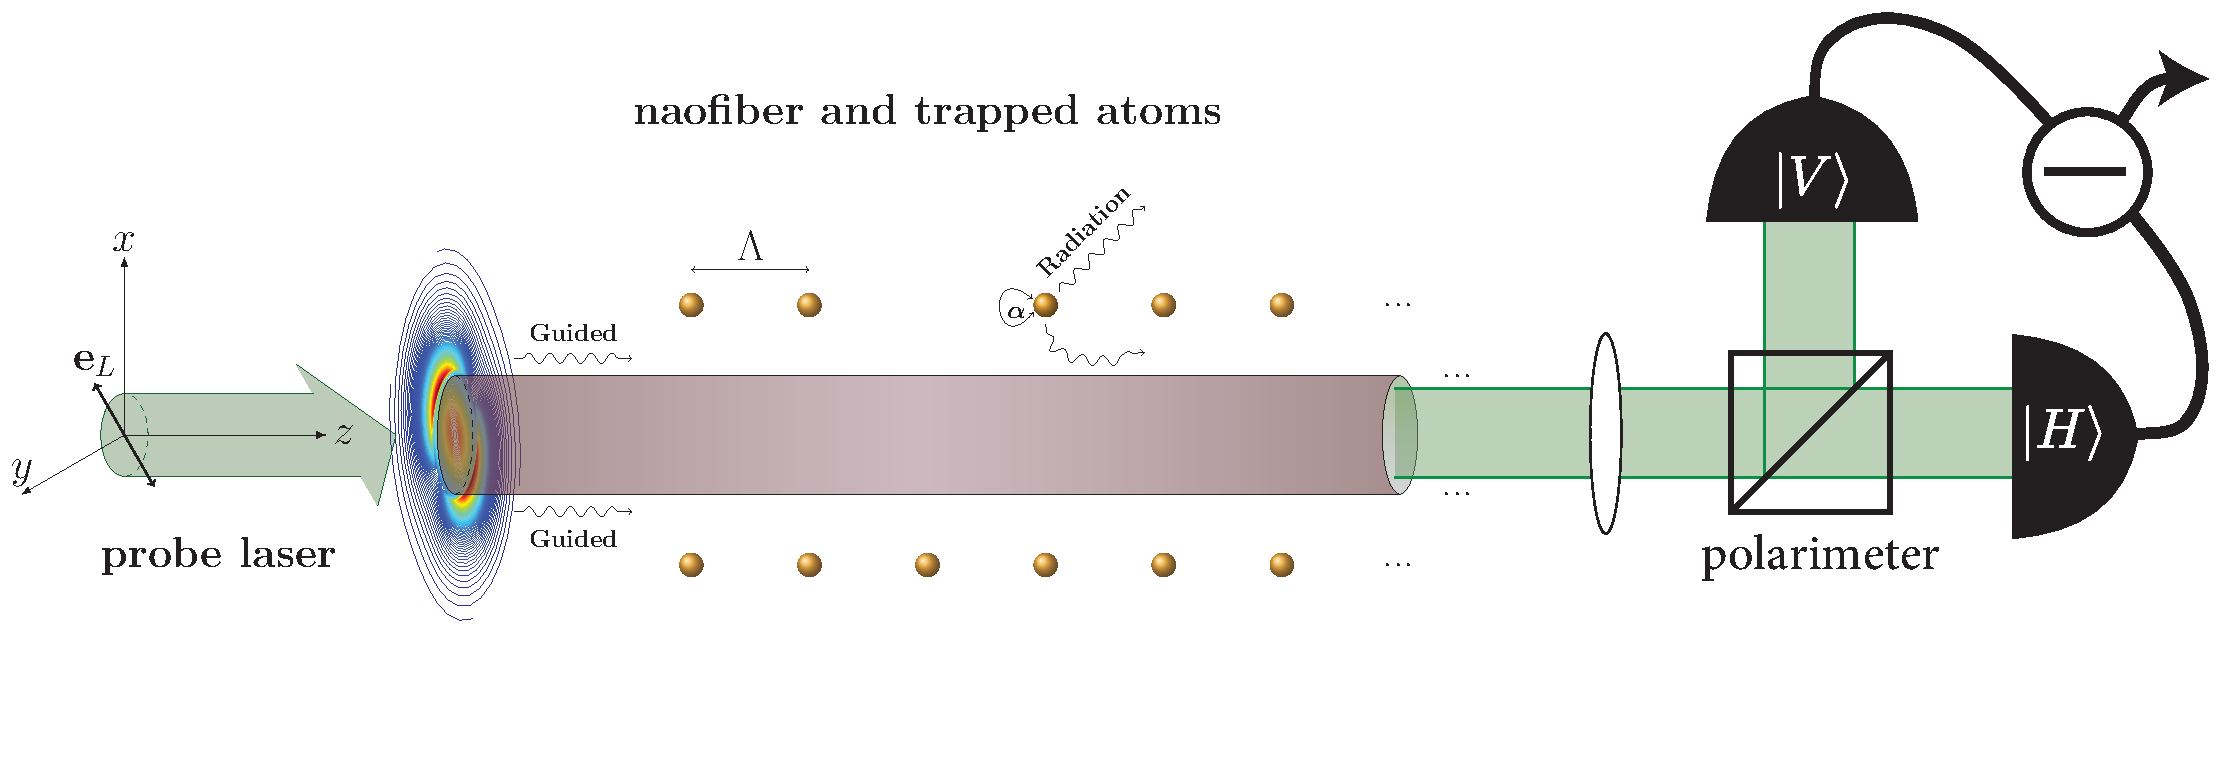
\includegraphics[scale=0.35]{./Figs/BirefringenceMeasurement_randomAtoms}
\caption{Birefringence measurement setup for a nanofiber trapped atomic system. In the evanescent 
field of the nanofiber, atoms (golden balls) randomly  occupy the periodic trapping sites on both sides of 
a 1D-chain with a period of $\Lambda$.}
\label{fig:BirefringenceMeasurement}
\end{figure}

\section{Dyadic Green's function and input-output field response}
The fundamental quantity that captures the modification of of atomic radiation near dielectric surfaces 
with index of refraction function, $n(\mbf{r})$, is the dyadic Green's function, defined by
 \begin{align}
\left[ -\nabla\times\nabla\times + n^2(\mbf{r}) k^2 \right] \tensor{\mathbf{G}}(\br, \br';\omega) &= -4 \pi 
k^2 \delta^{(3)}(\mathbf{r}-\mathbf{r}')\;\tensor{\mathbf{I}},
\end{align}
where $k=\omega/c$; Gaussian-cgs units are used throughout.  On resonance, at $\br=\br'$, 
$\Im\left(\tensor{\mathbf{G}}(\br', \br'; \omega= \omega_A) \right)$ determines the Purcell effect.  We 
seek here the off-resonance dispersive response.

Given a point particle at position $\br'$ with tensor polarizability $\tensor{\boldsymbol{\alpha}}$, the  
scattering solution to wave equation at frequency $\omega_0$
\begin{align}\label{eq:Maxwellwithsource2}
\left[\! -\! \nabla\!\!\times\!\nabla\!\!\times + n^2\!(\br)k_0^2 \right]\!\! \mathbf{E}(\br) &\!=\! -4\pi\! k_0^2 
\delta^{(3)}(\br-\br')\;  \tensor{\boldsymbol{\alpha}}\cdot \mathbf{E}(\br),
\end{align}
is given by the Lipmann-Schwinger equation
\begin{align}
\mathbf{E}_{out}(\br) &=\mathbf{E}_{in}(\br)+\tensor{\mathbf{G}}^{(+)}(\br , \br'; \omega_0)\cdot 
\tensor{\boldsymbol{\alpha}}\cdot \mathbf{E}_{out}(\br')\\
&\approx \mathbf{E}_{in}(\br)+ \tensor{\mathbf{G}}^{(+)}(\br , \br'; \omega_0) \cdot 
\tensor{\boldsymbol{\alpha}}\cdot \mathbf{E}_{in}(\br'),
\end{align}
where $\mathbf{E}_{in}(\br)$ is the asymptotic input field, $\tensor{\mathbf{G}}^{(+)}$ is the retarded 
Green's function solution, and in the second line we made the Born approximation valid for weak 
scattering.  

A complete solution for $\tensor{\mathbf{G}}(\br ,\br' ; \omega_0)$, following from Maxwell's equations 
has been studied previously [].  As we are interested here in the forward scattered component that 
leads to phase shifts and polarization transformations, we can directly calculate this through a 
decomposition into normal modes.  A complete set of eigenmodes in the presence of a dielectric are 
defined according to the procedure of Glauber and Lewenstein~\cite{Glauber1991}.  Define, 
$\tilde{\mathbf{F}}_\mu(\br) \equiv n(\br) \mathbf{F}_\mu (\br)$, where $\mathbf{F}_\mu (\br)$ is 
proportional to the electric field of the corresponding fiber modes.  These form a complete set of 
(transverse) vector functions as they are eigenfunctions of a Hermitian operator, 
$\tensor{\mathcal{H}}(k) = -\frac{1}{n(\br)}
\nabla\times\nabla\times \frac{1}{n(\br)} + k^2 \tensor{\mathbf{I}}$ according to 
$\tensor{\mathcal{H}}(k_0) \cdot \tilde{\mathbf{F}}_\mu = \lambda_\mu \tilde{\mathbf{F}}_\mu$, where 
$\lambda_\mu=k_0^2-k_\mu^2$.
The complete orthonormal modes thus satisfy,
\begin{align}
\int \tilde{\mathbf{F}}_\mu^* (\br)\cdot \tilde{\mathbf{F}}_{\mu'}(\br) \mathrm{d}^3\br &= \int n^2(\br) 
\mathbf{F}_\mu^* (\br)\cdot  \mathbf{F}_{\mu'}(\br) 
\mathrm{d}^3\br=\delta_{\mu\mu'},\label{eq:orthutrans}
\\
\sum_\mu \tilde{\mathbf{F}}_\mu (\br) \tilde{\mathbf{F}}_\mu^*(\br') &= \sum_\mu n(\br)n(\br') 
\mathbf{F}_\mu  (\br) \mathbf{F}_\mu^*(\br) =\tensor{\delta}^{(T)}(\br-\br'), 
\end{align}
where $\tensor{\delta}^{(T)}(\br-\br')$ is the  delta function for ``transverse" (divergenceless) vector 
fields.  It follows that the dyadic (transverse) Green's function can be decomposed as~\cite{Swedishguys}
\begin{equation}
\tensor{\mathbf{G}}(\br,\br'; \omega_0) = -4\pi \sum_{\mu} \frac{\omega_0^2\mathbf{F}_\mu (\br) 
\mathbf{F}^*_\mu (\br')}{\omega_0^2-\omega_\mu^2},
\end{equation}
where $\omega_\mu^2 = c^2 k_\mu^2$.  This sum separates into guided an unguided contributions. 

Given the cylindrical symmetry, the guided modes are defined, $\mathbf{F}_\mu (\br) = \mathbf{u}_\mu 
(\br_\perp) e^{i\beta z}$, where the mode index $\mu=\{n, \beta, p\}$ for the guided mode $n$, with 
polarization $p$.  These can be either quasilinear linear or quasicircular modes~\cite{?}, whose 
$z$-components satisfy the two-dimensional Schr\"{o}dinger-like equation, $\left[\nabla_T^2 +k_0^2 
n^2(r_\perp) \right] u_{\mu,z} (\br_\perp) = \beta^2 u_{\mu,z} (\br_\perp)$.  We treat here nanofibers, 
which support only the lowest HE$_{11}$ guided modes at frequency $\omega_0$, and thus we with 
drop the mode index $n$.  In this case there are only four guided modes with two polarizations $p$ and 
$\beta = \pm \beta_0$, corresponding to forward and backward propagation for the single bound field.  
The guided contribution to the dyadic Greens function is then 
\begin{equation}
\tensor{\mathbf{G}}_g(\br,\br'; \omega_0) = \int_{-\infty}^\infty \frac{d \beta}{2 \pi} \sum_{p} 
\frac{-4\pi\omega_0^2\mathbf{u}_{\beta,p} (\br\!_\perp)\mathbf{u}^*_{\beta,p} 
(\br_{\!\perp}^\prime)}{\omega_0^2-\omega^2(\beta)}e^{i\beta(z-z')},\label{eq:Gganaly}
\end{equation}
where $ \omega(\beta)$ is the frequency of the guided HE$_{11}$ for a given $\beta$.  Note, for the 
HE$_{11}$ mode there is no cutoff; for a given $\omega$, there is a guided mode with propagation 
constant $\beta(\omega)$.  

For $z>z'$ ($z>z'$), the contribution of the guided modes to the retarded Green's function is found by the 
usual displacement of the pole on the positive (negative) $\beta$-axis into the upper (lower) half of 
complex plane, and closing the contour, to yield
\begin{align}
\tensor{\mathbf{G}}^{(+)}_g(\br,\br'; \omega_0) &= 2\pi i \sum_{p}  {\rm Res}\vert_{\beta =\beta_0} 
\left[\frac{-4\pi \omega_0^2}{2\pi (\omega_0^2-\omega^2(\beta))}\right]  \mathbf{u}_{f\beta_0, p} 
(\br\!_\perp)\mathbf{u}^*_{f\beta_0, p} (\br_{\!\perp}^\prime)e^{if \beta_0 (z-z')} \nonumber \\
&  =  i 2\pi f \frac{\omega_0}{v_g } \sum_{p} \mathbf{u}_{f, p} (\br\!_\perp)\mathbf{u}^*_{f , p} 
(\br_{\!\perp}^\prime) e^{if \beta_0(z-z')}\;\; {\rm for }\;  (z-z')f>0,
\label{eq:Gganaly}
\end{align}
where $f=\pm 1$, $v_g= d\omega/d\beta \vert_{\beta=\beta_0}$ is the group velocity, and we suppressed 
the label $\beta_0$ as implicit in the definition of the guided mode at frequency $\omega_0$. For 
$\br=\br'$ we cannot close the contour. Instead, we expand the resonant denominator in Eq. () with the 
poles moved to yield the retard (causal) response,
\begin{equation}
\frac{1}{(\omega_0+i\epsilon)^2-\omega^2(\beta)}=\frac{1}{2 \omega(\beta)}\left[ \frac{1}{\omega_0+ i 
\epsilon - \omega(\beta)} - \frac{1}{\omega_0+ i \epsilon + \omega(\beta)} \right],
\end{equation}
 and employ the usual distribution identities,
\begin{equation}
\lim_{\epsilon \rightarrow 0_+} \frac{1}{\omega_0 + i \epsilon \mp 
\omega(\beta)}=\mathcal{P}\left[\frac{1}{\omega \mp \omega(\beta)} \right] + i \pi \delta (\omega_0 \mp 
\omega(\beta)).
\end{equation}
As only the positive frequency component contributes to the delta function, it follows that the imaginary 
part of the Green's function at $\br = \br'$ that determines the Purcell enhancement of spontaneous 
emission into the guided mode is
\begin{equation}
\Im\left[\tensor{\mathbf{G}}^{(+)}_g(\br',\br'; \omega_0) \right] = \pi \frac{\omega_0}{v_g } \sum_{f, p} 
\mathbf{u}_{f, p} (\br_{\!\perp}^\prime)\mathbf{u}^*_{f , p} (\br_{\!\perp}^\prime).
\end{equation}
The real part determines the level shift on the atom due to its proximity to the dielectric.

Equation (\ref{eq:Gganaly}) is the central result, from which we can calculate the dispersive response.  
Consider an input field with arbitrary polarization , $\mathbf{E}_{in}(\br) = \sum_p E_p 
\mathbf{u}_{+,p}(\br_\perp) e^{+i \beta_0 z}$ and an atom localized at $z'=0$.  Substituting Eq. 
(\ref{eq:Gganaly}) into Eq. (?) yields the transmitted (forward scattered) output field 
\begin{equation}
\mathbf{E}_{out}(\br) =  \sum_{p',p} t_{p'p} E_p \mathbf{u}_{+, p'}(\br_\perp) e^{+i \beta_0 z}, 
\end{equation}
where, for an atom located at $\br'_\perp$, the transmission matrix is
\begin{equation}
t_{p' p} = \delta_{p' p} + i 2\pi k_0 \frac{c}{v_g}\mathbf{u}^*_{+, p'}(\br'_\perp) \cdot 
\tensor{\boldsymbol{\alpha}} \cdot \mathbf{u}_{+, p}(\br'_\perp) .
\end{equation}
The diagonal terms determine the attenuation and phase shift induced on each polarization component 
according to $t_{p p} \approx \sqrt{1-R}e^{i \phi_p}$ where
\begin{align}
\delta \phi_p &= \frac{2 \pi k_0 \Re(\alpha_p) }{\tilde{A}} \frac{c}{v_g}, \\
R &=  \frac{4 \pi k_0 \Im(\alpha_p) }{\tilde{A}} \frac{c}{v_g},
\label{phaseshift} 
\end{align}
and 
\begin{equation}
 \frac{\alpha_p}{\tilde{A}} \equiv \mathbf{u}^*_{+,p}(\br'_\perp) \cdot \tensor{\boldsymbol{\alpha}}\cdot 
 \mathbf{u}_{+, p}(\br'_\perp). 
 \end{equation}
 The phase shift per atom is modified over free space in two ways.  The mode dispersion relation 
 $\omega(\beta)$ can lead to an enhancement due to a group velocity reduction. This factor is less 
 important for the nanofiber geometry under consideration here.  More importantly, the effective mode 
 area $\tilde{A} \sim |\mathbf{u}_{+,p}(\br'_\perp)|^{-2}$ is typically orders of magnitude smaller than 
 for a paraxial laser beam in free space.  
 
 The off-diagonal terms in the transmission matrix correspond to polarization transformations.  For 
 example, if we take the polarizations to be the quasilinear modes~\cite{?}, which we will denote $\{ 
 \mathbf{u}_{H}, \mathbf{u}_{V}\}$, then $t_{H,V} \equiv \chi_{Far}$,  the rotation angle of the Faraday 
 effect.  In this basis, the phase difference $\delta  \phi_H - \delta \phi_V$ corresponds to birefringence.  
 Alternatively, analyzed in the quasicircular polarization basis, $\delta \phi_+ -\delta  \phi_-$ corresponds 
 to Faraday rotation and $t_{+,-}$ to birefringence.  We will consider the use of such polarization 
 transformations as a means to measure atoms and perform collective spin squeezing.

\subsection{Heisenberg-Langevin picture solution and atomic response}
The Lippmann-Schwinger solution, Eq. (?) determines the input-output relation given linear atomic 
response as expressed by the polarizability tensor $\tensor{\alpha}$.  In this section we derive the 
dispersive atomic response and quantized mode input-ouput relations using the Heisenberg-Langevin 
picture for one-dimensional systems following the formalism laid out in~\cite{Haikuta}.  The positive 
frequency component of the quantized electric field decomposes into guided and radiative (unguided 
modes) according  $\hat{\mathbf{E}}^{(+)}=\hat{\mathbf{E}}_g^{(+)}+\hat{\mathbf{E}}_{r}^{(+)}$, where
\begin{align}
\hat{\mathbf{E}}_g^{(+)}(\br) &= \sum_{f,p} \int \mathrm{d}\omega \sqrt{\frac{ \hbar \omega}{v_g}} 
\hat{a}_\mu \mathbf{u}_\mu (\br\!_\perp) e^{if\beta z},\\
\hat{\mathbf{E}}_r^{(+)}(\br) &= \sum_{m,p} \int \mathrm{d}\omega  \int_{-kn_2}^{kn_2}\mathrm{d}\beta 
\sqrt{ \hbar \omega} \hat{a}_\nu \mathbf{u}_\nu (\br\!_\perp) e^{i\beta z},
\end{align}
where $\mu =(\omega, f, p)$ indexes the four HE$_{1,1}$ guided modes at a given $\omega$ (two 
polarizations $p$ and forward or backward propagation with wavenumber $f\beta (\omega)$, 
$f=\pm1$), and $\nu=(\omega, \beta, m, p)$ indexes the frequency, propagation constant, and azimuthal 
quantum number of the unguided modes, $m$.  The creation/annihilation operators satisfy the usual 
continuous mode commutation relations, $[\hat{a}_\mu, \hat{a}^\dag_{\mu'} ] = \delta_{p,p'} \delta_{f,f'} 
\delta ( \omega - \omega ') $, $[\hat{a}_\nu ,\hat{a}^\dag_{\nu'} ] = \delta_{p,p'} \delta_{m,m'} \delta ( 
\omega - \omega ')  \delta ( \beta - \beta') $.


The Hamiltonian for the system is
\begin{equation}
\hat{H} = \hat{H}_F+\hat{H}_A + \hat{H}_{int}.
\end{equation}
The free field Hamiltonian decomposes into guided and unguided modes, 
\begin{equation}
\hat{H}_0 = \sum_{f,p}\int \mathrm{d}\omega \hbar \omega \hat{a}^\dagger_\mu \hat{a}_\mu 
+\sum_{m,p} \int \mathrm{d}\omega  \int_{-nk_0}^{nk_0} \mathrm{d}\beta \hbar \omega 
\hat{a}^\dagger_\nu \hat{a}_\nu.
\end{equation}
We consider here alkali atoms with hyperfine multiplets of ground and excited levels, $\{ 
\ket{g}=\ket{nS_{1/2}, F, M_F}\}$, $\{ \ket{e} =\ket{nP_{J'}, F', M_{F'}}\}$,
\begin{equation}
\hat{H}_A  = \sum_g E_g \ket{g}\bra{g} + \sum_e E_e \ket{e}\bra{e}.
\end{equation}
In the rotating wave approximation, the atom-field interaction Hamiltonian is
\begin{align}
\hat{H}_{int} &= -\hat{\mathbf{d}}\cdot \hat{\mathbf{E}} = -\hat{\mathbf{d}}_{eg}\cdot 
\hat{\mathbf{E}}^{(+)}(\br')-\hat{\mathbf{d}}_{ge}\cdot \hat{\mathbf{E}}^{(-)}(\br'),
\end{align}
where the dipole operator is projected between excited and ground subspaces, $\hat{\mathbf{d}}_{eg}= 
\hat{P}_e \hat{\mathbf{d}} \hat{P}_g $. The interaction Hamiltonian then takes the form, 
\begin{equation}
\hat{H}_{int} = -\sum_{eg} \left(\sum_{f,p} \int\mathrm{d}\omega \; \hbar g_{\mu, e,g}\; \hat{a}_\mu  \; 
\hat{\sigma}_{e,g}+ \sum_{m,p} \int\mathrm{d}\omega \int_{-kn_2}^{kn_2}\mathrm{d}\beta \;  \hbar 
g_{\nu, e,g}\; \hat{a}_\nu \; \hat{\sigma}_{e,g}+  h.c.\right),
\end{equation}
where $\hat{\sigma}_{\alpha,\beta}= \ket{\alpha}\bra{\beta}$ are the atomic two-level operators, and 
the coupling constants between the electric dipole and the guided or radiative modes are
\begin{align}
\hbar g_{\mu, e,g} &= \sqrt{\frac{\hbar \omega}{v_g}}\; \bra{e} \hat{\mathbf{d}} \ket{g} 
\cdot\mathbf{u}_\mu (\br'), \\
\hbar g_{\nu, e,g} &= \sqrt{\hbar \omega} \; \bra{e} \hat{\mathbf{d}} \ket{g} \cdot \mathbf{u}_\nu (\br') .
\end{align}
The Heisenberg equations of motion thus follow,
\begin{align}
\dt{\hat{a}_\mu} &= -i\omega \hat{a}_\mu +i\sum_{eg} g_{\mu, e,g}^* \hat{\sigma}_{g,e} \label{eq:da}\\
\dt{\hat{a}_\nu} &= -i\omega \hat{a}_\nu +i\sum_{eg} g_{\nu, e,g}^*  \hat{\sigma}_{g,e} \label{eq:danu}\\
\dt{\hat{\sigma}_{ge}} &= -i\omega_{eg} \hat{\sigma}_{g,e} \nonumber\\
&+ i\int_0^{\infty}\mathrm{d}\omega \sum_{e'g'} \left[ (\delta_{ee'} \hat{\sigma}_{gg'} - \delta_{gg'} 
\hat{\sigma}_{e'e}) \left\{ \sum_{f,p}  g_{\mu, e',g'}\hat{a}_\mu +\sum_{m,p}  
\int_{-kn_2}^{kn_2}\mathrm{d}\beta \; g_{\nu, e',g'} \hat{a}_\nu \right\}   \right]
 \label{eq:dsigma} 
\end{align}
Integrating the field equations, 
\begin{subequations}\label{eq:aout1}
\begin{align}
\hat{a}_\mu(t) &= \hat{a}_\mu(t_0) e^{-i\omega (t-t_0)} +i \sum_{e,g} g_{\mu,e,g}^* \int_{t_0}^t 
\mathrm{d} t' e^{-i\omega (t-t')}\hat{\sigma}_{g,e}(t')
\end{align}
\begin{align}
\hat{a}_\nu (t) &= \hat{a}_\nu (t_0) e^{-i\omega (t-t_0)} +i \sum_{eg} g_{\nu,e,g}^* \int_{t_0}^t \mathrm{d} 
t' e^{-i\omega (t-t')}\hat{\sigma}_{g,e}(t'),
\end{align}
\end{subequations}
and substituting into Eq. (?), in the Markoff approximation~\cite{?} yields
\begin{align}
&\dt{\hat{\sigma}_{g,e}} =-i\omega_{eg} 
\hat{\sigma}_{g,e}-\sum_{e'}\frac{\Gamma_{ee'}}{2}\hat{\sigma}_{g,e'} \nonumber \\
&+i \sum_{e'g'}\left[ (\delta_{ee'} \hat{\sigma}_{gg'} - \delta_{gg'} 
\hat{\sigma}_{e'e})\int_0^{\infty}\mathrm{d}\omega \left\{\sum_{f,p}  g_{\mu, e',g'}\; \hat{a}_\mu (t_0) 
+\sum_{m,p}  \int_{-kn_2}^{kn_2}\mathrm{d}\beta \; g_{\nu, e',g'} \;\hat{a}_\nu(t_0)   \right\} e^{-i\omega 
(t-t_0)}\right]
\end{align}
where 
\begin{equation}
\Gamma_{ee'} = 2\pi \sum_{f,p,g} g_{\mu,e,g}g^*_{\mu,e',g} \vert_{\omega=\omega_{eg}}+2\pi 
\sum_{m,p,g'} g_{\nu,e,g}g^*_{\nu,e',g'} \vert_{\omega=\omega_{eg}}.
\end{equation}
The first sum represents decay into the guided mode while the second into the unguided radiation 
modes.  The total spontaneous emission rate of a given excited state into the guided modes is
\begin{equation}
\Gamma_e^{1D}= 2\pi \sum_{f,p,g} |g_{\mu,e,g}|^2_{\omega_{eg}} =  \sum_{f,p,g}\frac{2 \pi 
|\bra{e}\hat{\mathbf{d}}\ket{g} \cdot \mathbf{u}_{fp}(\br'_\perp)|^2}{\hbar} 
\left(\frac{\omega_{eg}}{v_g}\right).
\end{equation}
This agrees with the expected expression~\cite{?} following from the guided mode contribution to the 
dyadic Green's function, Eq. (?),
\begin{equation}
\Gamma_e^{1D} = \sum_{g}   \frac{2}{\hbar} \; \bra{g}\hat{\mathbf{d}}\ket{e}\cdot 
\Im\left(\tensor{\mathbf{G}}^{(+)}_g(\br', \br'; \omega= \omega_A) \right) \cdot 
\bra{e}\hat{\mathbf{d}}\ket{g},
\end{equation}
enhanced over the free space rate by the Purcell factor. 

Here we are interested in linear response, for excitation far from resonance.  In steady state, the dipole 
operator in the linear regime ($\hat{\sigma}_{e,e'} \rightarrow 0 $) is approximately
\begin{equation}
\hat{\sigma}_{g,e} =  -\sum_{g'} \hat{\sigma}_{g,g'}\int_0^{\infty}\mathrm{d}\omega \left(\sum_{f,p}  
\frac{g_{\mu, e,g'}}{\omega-\omega_{eg}}\; \hat{a}_\mu (t_0)+\sum_{m,p}  
\int_{-kn_2}^{kn_2}\mathrm{d}\beta \; \frac{g_{\nu, e,g'}}{\omega-\omega_{eg}} \;\hat{a}_\nu (t_0)  
\right)e^{-i\omega (t-t_0)} .
\end{equation}
By substituting this into Eq. (?), defining asymptotic modes, $\hat{a}^{in}(\omega) = \lim_{t_0\rightarrow 
-\infty} \hat{a}(t_0) e^{i\omega t_0}$, $\hat{a}^{out}(\omega) = \lim_{t\rightarrow +\infty} \hat{a}(t) 
e^{i\omega t}$ we obtain the input-output relationships of the guided modes due to the presence of an 
atom close to the nanofiber,
\begin{equation}
\hat{a}^{out}_\mu (\omega) = \hat{a}^{in}_\mu (\omega) \!-\! i\sum_{p',f'} 
\sum_{e,g,g'}\!\hat{\sigma}_{gg'}\frac{2\pi g_{\mu,e,g}^* 
g_{\mu',e,g'}}{\Delta_{eg}}\hat{a}^{in}_{\mu'}(\omega) \!-\! i\sum_{m,p} 
\sum_{e,g,g'}\!\hat{\sigma}_{gg'}\frac{2\pi  g_{\mu,e,g}^* 
g_{\nu',e,g'}}{\Delta_{eg}}\hat{a}^{in}_{\nu}(\omega).
\end{equation}
This agrees with the expected form given by the Lipmann-Schwinger Equation in the first Born 
approximation,
\begin{equation}
\hat{\mathbf{E}}^{(+)}_{g,out}(\br)=\hat{\mathbf{E}}^{(+)}_{g, 
in}(\br)+\tensor{\mathbf{G}}_g^{(+)}(\br,\br',\omega)\cdot\hat{\tensor{\alpha}}\cdot 
\left(\hat{\mathbf{E}}^{(+)}_{g, in}(\br')+\hat{\mathbf{E}}^{(+)}_{r, in}(\br')\right),
\end{equation}
by noting
\begin{equation}
 \mathbf{u}_{\mu} (\br)\cdot \tensor{\mathbf{G}}_g^{(+)}(\br,\br',\omega)\cdot 
 \hat{\tensor{\boldsymbol{\alpha}}}\cdot \mathbf{u}_{\mu'} (\br') = i 2\pi k\frac{c}{v_g} \mathbf{u}_\mu 
 (\br) \cdot \hat{\tensor{\boldsymbol{\alpha}}}\cdot \mathbf{u}_{\mu'} (\br') = - i \sum_{e,g,g'}\!\ 
 \hat{\sigma}_{gg'} \frac{2\pi g_{\mu,e,g}^* g_{\mu',e,g'}}{\Delta_{eg}},
\end{equation}
where the dyadic Green's function is give in Eq. (?) and the atomic polarizability tensor operator is
\begin{equation}
\hat{\tensor{\boldsymbol{\alpha}}} = -\sum_{e,g,g'}\ket{g}\frac{\bra{g}\hat{\mathbf{d}}\ket{e}\bra{e} 
\hat{\mathbf{d}}\ket{g'}}{\hbar \Delta_{eg}}\bra{g'}.
\end{equation}
Scattering of classical waves follows when the field is in a coherent state.  The phase-shift on a guided 
mode with a given polarization $p$, Eq. (?), now depends on the internal state of the atom.  Given atoms 
in a particular ground sublevel $\ket{g}$, this can be expressed
\begin{equation}
\delta  \phi_{p,g} =2\pi k_0 \frac{c}{v_g}\mathbf{u}^*_{+, p}(\br'_\perp) \cdot \bra{g} 
\hat{\tensor{\boldsymbol{\alpha}}} \ket{g} \cdot \mathbf{u}_{+, p}(\br'_\perp) = -\sum_e \frac{2 \pi 
|\bra{e}\hat{\mathbf{d}}\ket{g} \cdot \mathbf{u}_{+,p}(\br'_\perp)|^2}{\hbar \Delta_{eg}} 
\left(\frac{\omega}{v_g}\right).
\end{equation}

In relation to Eq. (?) we see that $\delta \phi \propto (\sigma_0/\tilde{A}) (\Gamma_{1D}/\Delta)$, where 
$\sigma_0$ is the resonant scattering cross section, and $\tilde{A}$ is the effective mode area defined in 
Eq. (?).  For comparison, the phase shift on a paraxial laser beam for an atom in vacuum has the same 
form as Eq. (?), but with the guided mode replaced by the  $\mathrm{TEM}_{00}$ mode of a Gaussian 
laser field at the atom position, with area $A=\frac{\pi w_0^2}{2}$. The strongest phase shift in free 
space is achieved when the atom is placed at the center of the beam waist.   The relative strength of the 
phase shift is $\delta \phi_{nano}/\delta \phi_{vac}\propto (A/\tilde{A}) (c/v_g)$, as plotted in Fig. ? as a 
function of the position of the atom.  For example, for a quasilinear field, and an atom trapped along the 
direction of the input polarization  at $r_\perp = ?$, $\delta \phi_{nano}/\delta \phi_{vac} = ?$.   Thus we 
see that, in the nanofiber geometry the Purcell factor does not cause the majority of scattering to be 
guided, nor is the phase shift enhanced greatly over the phase shift imparted by an atom at the center of 
a paraxial beam.  However, the key feature is that this phase shift will add directly for a chain of atoms 
trapped along the fiber.  Thus one can achieve an effective optical density in the fiber geometry with 
moderate ensembles ($\sim 1000$ atoms) that would require $\sim 10^6$ atoms in free space.  The 
result is much larger average entangling interaction/atom whose application in QND measurement we 
explore below.

\missingfigure{Figure for the enhancement comparison.}


\section{QND measurement of atoms}
The dispersive interaction between the atoms and nanofiber guided photons provides a mechanism with which to perform a QND measurement on the atoms.  We take the atoms to be trapped along the $x$-axis at position $(r'_\perp =a, \phi' =0)$.  We restrict here to two quasi-linear polarizations, $\mu =\{H,V\}$, of the single HE$_{11}$ guided mode propagating in the positive $z$-direction.  Outside the fiber, the transverse mode functions are~\cite{?}
\begin{align}
u_{H,x}(r_\perp,\phi) &= u_0 \frac{\beta_0}{2 q}[(1-s)K_0(q r_\perp) - (1+s)K_2(q r_\perp) \cos(2 \phi)], \\
u_{H,y}(r_\perp,\phi) &=-u_0 \frac{\beta_0}{2 h}  (1+s)K_2(q r_\perp) \sin(2 \phi) ,\\
u_{H,z}(r_\perp,\phi) &=iu_0 \frac{J_1(ha)}{K_1{qa}} K_1(q r_\perp) \cos(\phi), \\
u_{V,x}(r_\perp,\phi) &= u_0 \frac{\beta_0}{2 q}(1+s)K_2(q r_\perp) \sin(2 \phi)] ,\\
u_{V,y}(r_\perp,\phi) &=u_0 \frac{\beta_0}{2 h} [(1-s)K_0(q r_\perp) - (1+s)K_2(q r_\perp) \cos(2 \phi)], \\
u_{V,z}(r_\perp,\phi) &=iu_0 \frac{J_1(ha)}{K_1{qa}}K_1(q r_\perp) \sin(\phi), 
\end{align}
where $u_0$ is set by the normalization condition, $\int d^2 r_\perp n(r_\perp) | \mathbf{u}_\mu(\br_\perp)|^2=1$, $J_n$ and $K_n$ are Bessel functions of the first and second kind, $h=\sqrt{n^2 k_0^2 - \beta_0^2}$, $q=\sqrt{\beta_0^2- k_0^2}$, and $s = [(q a)^{-2} + (h a)^{-2}]/[J'_1(ha)/haJ_1(ha) + K'_1(qa)/qaK_1(qa)]$.  Note, the $\mathbf{u}_H$ and $\mathbf{u}_y$ adiabatically connect through the fiber taper to $x$- and $y$-linearly polarized plane wave modes.  In the nanofiber region $\mathbf{u}_H$ is purely $x$-polarized at $\phi = \phi/2$ and the  $\mathbf{u}_V$ is purely $y$-polarized at $\phi = 0$.  At all other $\phi$ the electric field is generally rotating along an ellipse.  


The Lipmann-Schwinger input-ouput scattering equation, Eq. (?), follows in the time domain as the evolution of coarse-grained time modes.  For each  $\mu =\{H,V\}$, HE$_{11}$ mode, we define propagating annihilation operators~\cite{},
\begin{equation}
\hat{a}_\mu(z,t) = \int \frac{d \omega}{\sqrt{2 \pi}} \; \hat{a}_\mu e^{i(n_\mu(\omega) kz-\omega t)},
\end{equation}
satisfying free field commutation relations
\begin{equation}
\left[\hat{a}_\mu(z,t),\hat{a}^\dag_\nu(z',t')\right]=\delta_{\mu,\nu}  \delta(t-t'-(z-z')/v_g).
\end{equation}
The quantized electric field operator for these guided modes, Eq. (?), is then
\begin{equation}
\hat{\mathbf{E}}^{(+)}(r\!_\perp,\phi,z;t) = \sqrt{ \frac{2 \pi \hbar \omega_0}{ v_g} } \big( \mathbf{u}_H(r\!_\perp,\phi) \hat{a}_H(z,t) + \mathbf{u}_V(r\!_\perp,\phi) \hat{a}_V(z,t) \big) e^{i \beta_0 z},
\end{equation}
whose interaction with atoms in the dispersive regime is governed by  light-shift Hamiltonian~\cite{Deutsch2010a}
\begin{equation}  
	\hat{H}_{LS}   = - \sum_i \hat{\mathbf{E}}^{(-)}(\mathbf{r}'_i ; t ) \cdot \hat{\tensor{\boldsymbol{\alpha}}}(i) \cdot \hat{\mathbf{E}}^{(+)}(\mathbf{r}'_i;t ).
\end{equation}
Here $\hat{\tensor{\boldsymbol{\alpha}}}(i)$ is the polarizability tensor operator, Eq. (?), for an atom trapped near the nanofiber surface at position $\mathbf{r}'_i$. The Hamiltonian thus takes the form,
\begin{align}  
	\hat{H}_{LS}   &= -\frac{2 \pi \hbar \omega_0}{v_g} &\sum_i &\sum_{\mu,\nu} \hat{\alpha}_{\mu \nu}\; \hat{a}_{\mu}^\dag(z_i,t)  \hat{a}_{ \nu}(z_i,t) \\
	&= -\frac{2 \pi \hbar \omega_0}{v_g} &\sum_i &  \left[\hat{\alpha}_{HH}+\hat{\alpha}_{VV} \right]_i \hat{S}_0(z_i,t) +  \left[\hat{\alpha}_{HH}-\hat{\alpha}_{VV} \right]_i \hat{S}_1(z_i,t) \nonumber \\
	&&+ &\left[\hat{\alpha}_{HV}+\hat{\alpha}_{HV} \right]_i \hat{S}_2(z_i,t) + i  \left[\hat{\alpha}_{HV}-\hat{\alpha}_{VH} \right]_i \hat{S}_3(z_i,t)  \nonumber \\
	\end{align}
where
\begin{equation}  
\hat{\alpha}_{\mu \nu}(i)= \mathbf{u}^*_\mu(r'_{\perp i},\phi'_i)  \cdot \hat{\tensor{\boldsymbol{\alpha}}}(i) \cdot \mathbf{u}_\nu(r'_{\perp i},\phi'_i),
\end{equation}
and 
\begin{align}
\hat{S}_1(z,t) = \frac{1}{2}\left(\hat{a}^\dag_H \hat{a}_H-\hat{a}^\dag_V \hat{a}_V \right), \; \hat{S}_2(z,t) = \frac{1}{2}\left(\hat{a}^\dag_H \hat{a}_V+\hat{a}^\dag_V \hat{a}_H \right), \; \hat{S}_3(z,t) = \frac{1}{2i}\left(\hat{a}^\dag_H \hat{a}_V-\hat{a}^\dag_V \hat{a}_H \right) 
\end{align}
are the propagating components of the Stokes vector operator, satisfying commutation relations
\begin{equation}
\left[\hat{S}_i(z,t), \hat{S}_j(z,t')\right] =i \epsilon_{ijk} \hat{S}_k(z,t) \delta(t-t').
\end{equation}
We round out the definitions with 
\begin{equation}
\hat{S}_0(z,t) = \frac{1}{2}\left(\hat{a}^\dag_H \hat{a}_H+\hat{a}^\dag_V \hat{a}_V \right), 
\end{equation}
which represents the total flux of photons propagating in the guided mode.

 
We explore a QND measurement of cesium atoms in the hyperfine manifold of the electronic ground state, $6S_{1/2}$ via polarization spectroscopy.  The polarizability tensor decomposes into irreducible components depending on detuning near the D1 or D2 resonance $6P_{J'}$,
\begin{align}
\hat{\alpha}_{ij} &= \hat{\alpha}_{ij}^{(0)}(F',F)+\hat{\alpha}_{ij}^{(1)}(F',F)+\hat{\alpha}_{ij}^{(2)}(F',F)\\
&=\sum_{F,F'} \alpha_0 \left[ C_{J'FF'}^{(0)} \delta_{ij}+ iC_{J'FF'}^{(1)}\epsilon_{ijk}\hat{F}_k+ C_{J'FF'}^{(2)}\left(\frac{1}{2} ( \hat{F}_i\hat{F}_j +\hat{F}_j\hat{F}_i )-\frac{1}{3}\hat{\mathbf{F}}^2 \delta_{ij} \right) \right],
\end{align}
where $\hat{\mathbf{F}}$ is the hyperfine spin operator, $\alpha_0 = -(\sigma_0/8\pi k_0) (\Gamma/\Delta_{F'F})$ is the characteristic dynamic polarizability for a scattering cross section $\sigma_0 = 3 \lambda^2/2\pi$, and $C_{J'FF'}^{(K)}$ are the tensor expansion coefficients~\cite{?}.  The nanofiber geometry gives rise to unique features of polarization spectroscopy not appearing in free space.  In addition to the polarization-dependent phase shifts arising from the atomic polarizability tensor in Eq. (?), the anisotropy of the  intensity for quasi-linearly polarized guide modes  leads to anisotropic atomic scattering of the $H$ and $V$ modes, giving rise to intrinsic birefringence, even for a purely scalar atomic polarizability.  In particular, choosing the quasi-$H$ axis, along the radial direction of the trapped atom leads to a phase delay of this mode relative the fast quasi-V axis.  This birefringence was exploited by Dawkins {\em et al.}~\cite{?} as mechanism implementing a QND measurement of the number of atoms trapped around the nanofiber, as we treat here.

Consider $N_A$ atoms, each in a completely mixed state.  In that case the $\langle \hat{\alpha}_{ij} \rangle = \sum_{F,F'} \alpha_0 C_{J'FF'}^{(0)} \delta_{ij}$.  With atoms trapped along the quasi-H axis,  $\langle \hat{\alpha}_{HV} \rangle = \langle \hat{\alpha}_{HV} \rangle =0$, but  $\langle \hat{\alpha}_{HH} \rangle \neq  \langle \hat{\alpha}_{VV} \rangle$.  The resulting Hamiltonian, Eq. (?), takes the form
\begin{equation}
\hat{H} = -2\pi \hbar  n_g k_0 N_A \left(\hat{\alpha}_{HH} - \hat{\alpha}_{VV}\right) =\hbar \chi N_A \hat{S}_1(0,t),
\end{equation}
where we have excluded the coupling to $\hat{S}_0$, which plays no role in the polarization spectroscopy, and have neglected the retardation associated with the different positions of the atoms along $z$.  The rotation angle on the Poincar\'{e} sphere is
\begin{equation}
\chi = n_g  \frac{\sigma_0}{\tilde{A}}  \sum_{F,F'}  C_{J'FF'}^{(0)} \frac{\Gamma}{4 \Delta_{F'F}}.
\end{equation}
where we have defined $\tilde{A}^{-1} \equiv |\mathbf{u}_{H}(\br'_\perp)|^2 - |\mathbf{u}_{V}(\br'_\perp)| ^2 $ as the inverse the effective area that characterizes the birefringence coupling constant. The effective optical density per atom is $\sigma_0/\tilde{A}$.  {\color{red}  Give some characteristic numbers.}  

To use this interaction to measure $N_A$, Dawkins {\em et al.} launched linearly polarized light at 45$^\circ$, i.e. along the Stoke $S_2$ axis, and measured the $S_3$ output component according to the input-output relation dictated by Hamiltonian Eq(?),
\begin{equation}
\hat{S}_3^{\rm out} = \hat{S}_3^{\rm in} + N_A \hat{S}_2^{\rm in}.
\end{equation}
The minimum atom number detectable by this type of QND measurement is set by the shot noise is the probe, i.e.,
\begin{equation}
\chi N_{\rm A, min} \langle \hat{S}_2^{\rm in}\rangle =  \langle \Delta \hat{S}_3^{\rm in}\rangle,
\end{equation}
where $\langle \hat{S}_2^{\rm in}\rangle  =N_L/2$ in the input Stokes vector magnitude and  $\langle  \Delta\hat{S}_3^{\rm in}\rangle = \sqrt{N_L/2}$ is the input shot noise rms for $N_L = P_{\rm in}\tau/\hbar\omega$ photons, given an input power, $ P_{\rm in}$.  This resolution is determined by the integration time of the signal, $\tau$, which in turn is limited by photon scattering into reflected and unguided modes. As a coarse approximation, we take this time to be $\tau=\gamma_s^{-1}$, where $\gamma_s$ is the photon scattering rate in free space.  For a detuning $\Delta$ large compared to the hyperfine splitting on the D2 line, $\gamma_s \hbar \omega_0=  \sigma \frac{\Gamma^2}{4 \Delta^2}\frac{P_{\rm in}}{A_{\rm in}}$, where $\sigma = (2/3) \sigma_0$ is the resonant scattering cross section arising from the scalar polarizability and $A_{\rm in}=|\mathbf{u}_{H}(\br'_\perp)|^{-2}$ is the effective area defined by the input intensity at the position of the atom.  The rotation angle, $\chi =n_g  \frac{\sigma}{\tilde{A}}\frac{\Gamma}{2\Delta}$.  Thus, the minimum detectable number of atoms within the shot-noise resolution is on the order of
\begin{equation}
N_{\rm A, min} = \frac{1}{\chi}\sqrt{\frac{2}{N_L}} = n_g \sqrt {\frac{A_{\rm in}}{\sigma}} \frac{  2 \sqrt{2}}{1-r},
\end{equation}
where the ratio $r \equiv |\mathbf{u}_{V}(\br'_\perp)| ^2/|\mathbf{u}_{H}(\br'_\perp)|^2$ characterizes the birefringence. {\color{red}  Give numbers}.

The same birefringent interaction can be employed in a QND measurement to squeeze the projection noise of the collective spin degrees of freedom of the atom ensemble.  In particular, consider squeezing of the uncertainty associated with the ``clock transition" of cesium.  Defining $\ket{\uparrow} = \ket{6S_{1/2}, F=4, M=0}$ and $\ket{\downarrow} = \ket{6S_{1/2}, F=3, M=0}$, the quantum uncertainty in the collective pseudo-spin $J_3 = \sum_{i=1}^{N_A} \sigma_z^{(i)}/2$ fundamentally limits the precision of atomic clocks.  Consider, the Hamiltonian, Eq. (?), but now restrict to the clock-state subspace. Again the  rank-1 ``vector light shift" vanishes since $\langle \uparrow | \hat{F}_k |\uparrow \rangle =\langle \downarrow | \hat{F}_k |\downarrow \rangle = 0$ for any choice of quantization axis. Thus, the terms in the Hamiltonian that give rise to Faraday effect vanish, leaving only birefringent coupling. The resulting Hamiltonian takes the form
\begin{align}
\hat{H}_{LS} = \hbar \Big\{ & \left[ \big( \chi_{H,\uparrow} +\chi_{V,\uparrow} \big) + \big( \chi_{H,\downarrow}+ \chi_{V,\downarrow}\big) \right] \frac{N_A}{2} \hat{S}_0 \nonumber \\
+ & \left[ \big( \chi_{H, \uparrow} - \chi_{V,\uparrow} \big) + \big(\chi_{H,\downarrow} - \chi_{V,\downarrow} \big)\right]  \frac{N_A}{2}\hat{S}_1 \nonumber \\
+ & \left[ \big( \chi_{H,\uparrow} +\chi_{V,\uparrow} \big) - \big( \chi_{H,\downarrow} + \chi_{V,\downarrow}\big) \right] \hat{J}_3 \hat{S}_0 \nonumber \\
+ & \left[  \big( \chi_{H, \uparrow} - \chi_{V,\uparrow} \big) - \big(\chi_{H,\downarrow} - \chi_{V,\downarrow} \big) \right]  \hat{J}_3 \hat{S}_1\Big\},
\end{align}
where 
\begin{equation}
\chi_{\mu,F} = - 2\pi n_g k_0 \bra{F,0}\hat{\alpha}_{\mu \mu}  \ket{F,0}
\end{equation}
is the rotation angle on the Poincar\'{e} sphere for an atom in the clock state with $F=4,3$ labeling $\uparrow,\downarrow$ and photon with polarization $\mu = H,V$. 


The first term in the Hamiltonian, Eq. (?), is an overall scalar shift and thus does not contribute to the relative dynamics.  The second term is a constant birefringence, independent of the atomic state, that we discussed above in the QND measurement of atom number.  In the context of squeezing, it can be canceled with a compensating waveplate as long as the atom number remains constant. The third term does not affect polarization spectroscopy, but will act to rotate the pseudo-spin around the $\mathbf{3}$-axis of the Bloch sphere.  While this does not affect the squeezing of project noise in $J_3$, it adds to uncertainty in the mean spin direction, which affects the metrologically relevant squeezing.   This term can, however, be canceled by choosing a ``magic wavelength" at which the light shift on $\ket{\uparrow}$ equals that on $\ket{\downarrow}$, i.e., 
$\chi_{H,\uparrow} +\chi_{V,\uparrow}  = \chi_{H,\downarrow} + \chi_{V,\downarrow}.$ The remaining QND interaction Hamiltonian is
\begin{equation}
\hat{H}_{LS} = \hbar \chi_{eff} \hat{J}_3 \hat{S}_1,
\end{equation}
where $\chi_{eff} = \big( \chi_{H, \uparrow} - \chi_{V,\uparrow} \big) - \big(\chi_{H,\downarrow} - \chi_{V,\downarrow} \big) = 2(\chi_{H, \uparrow}-\chi_{H, \downarrow})$ is the effective rotation angle at the magic wavelength.

The magnitude of the coupling angle, $\chi_{eff}$ depends on the maximizing the difference in the response of the atom to $H$ and $V$ modes in a way that depends on its spin-state.  This response will depend on the quantization axis that defines the clock state with projection $M=0$.  We obtain an compact expression for this by using the irreducible tensor decomposition of the atomic polarizability, Eq. (?).  Let $\mathbf{e}_\pi$ define the quantization axis and $\mathbf{e}_{1}$, $\mathbf{e}_{2}$ define two orthogonal linear $\sigma$ polarizations.  Then, because of the azimuthal symmetry of clock state around the $\mathbf{e}_\pi$ axis, the polarizability tensor is diagonal in the basis.  Note, $\langle F,0 | \hat{F}_{\pi}^2| F,0 \rangle =0$, $\langle F,0 | \hat{F}_{1}^2| F,0 \rangle = \langle F,0 | \hat{F}_{2}^2| F,0 \rangle = \langle F,0 | \hat{\mathbf{F}}^2| F,0 \rangle /2 =F(F+1)/2$.  It thus follows that the expectation value of the  irreducible rank-2 polarizability tensor is
\begin{equation}
\langle F,0 | \hat{\tensor{\boldsymbol{\alpha}}}^{(2)}| F,0 \rangle  = -\frac{\sigma_0}{8\pi k_0} F(F+1) \left\{ \frac{\tensor{\boldsymbol{1}} - 3 \mathbf{e}_\pi \mathbf{e}_\pi }{6} \right\} \sum_{F'} C^{(2)}_{J'F'F} \frac{\Gamma}{ \Delta_{F'F}},
\end{equation}
and from Eq. (?),
\begin{align}
\chi_{\mu,F} &= n_g \sigma_0 \sum_{F'}  \left\{C^{(0)}_{J'F'F}\left|\mathbf{u}_\mu(\br'_\perp)\right|^2+ C^{(2)}_{J'F'F} \frac{F(F+1)}{6}\left[\left|\mathbf{u}_\mu(\br'_\perp)\right|^2- 3 \left|\mathbf{e}_\pi \cdot \mathbf{u}_\mu(\br'_\perp)\right|^2 \right]\right\}   \frac{\Gamma}{4 \Delta_{F'F}} \nonumber \\
&  = n_g \sigma_0\left(  a_{F} \left|\mathbf{u}_\mu(\br'_\perp)\right|^2 + b_{F} \left|\mathbf{e}_\pi \cdot \mathbf{u}_\mu(\br'_\perp)\right|^2 \right),
\end{align}
where
\begin{equation}
a_F = \sum_{F'}  C^{(0)}_{J'F'F} \frac{\Gamma}{4 \Delta_{F'F}},\; \;\; b_F = \frac{F(F+1)}{6}\sum_{F'} C^{(2)}_{J'F'F}  \frac{\Gamma}{4 \Delta_{F'F}}.
\end{equation}
Birefringence arises from the first term due to the anisotropy of the intensity of the $H$ and $V$ modes and in the second term due to the anisotropy of tensor atomic response, which depends on the quantization axis of the atom.  At the magic wavelength the effective rotation angle $\chi_{eff}$ can then be written
\begin{equation}
\chi_{eff} = n_g\frac{\sigma_0}{A_{eff}} \frac{\Gamma}{4\Delta_{eff}}
\end{equation}
where
\begin{equation} 
\frac{\Gamma}{4\Delta_{eff}} = b_5 - b_4 = \sum_{F'}  \left( C^{(2)}_{J'F'5}\frac{5\Gamma}{4\Delta_{F',5}} -  C^{(2)}_{J'F'4}\frac{5\Gamma}{6 \Delta_{F',4} } \right),
\end{equation}
and
\begin{equation}
\frac{1}{A_{eff}} = \frac{\left|\mathbf{e}_\pi \cdot \mathbf{u}_H(\br'_\perp)\right|^2 \left|\mathbf{u}_V(\br'_\perp)\right|^2 - 
\left|\mathbf{e}_\pi \cdot \mathbf{u}_V(\br'_\perp)\right|^2 \left|\mathbf{u}_H(\br'_\perp)\right|^2}
{ \left|\mathbf{u}_H(\br'_\perp)\right|^2 +\left|\mathbf{u}_V(\br'_\perp)\right|^2 }.
\end{equation}
The quantization axis that maximizes $\chi_{eff}$ is that which minimizes $A_{eff}$.


\missingfigure{Poincare sphere diagram with spin squeezing effect.}

\missingfigure{Plots for $N^{min}_A$.}

\subsection{Other applications?} 


\section{Discussions}



%\begin{center}
%{\bf References}
%\end{center}

%\bibliography
%\bibliographystyle{amsplain}
\bibliographystyle{unsrt}
\bibliography{NanofiberArchive}
% \nocite{*}
%\ifwindows
%	\bibliography{F:/References/Archive/Archive}
%\else
%	\bibliography{/media/F/References/Archive/Archive}
%\fi


\end{document}